\documentclass{article}

% if you need to pass options to natbib, use, e.g.:
 \PassOptionsToPackage{numbers, compress}{natbib}
% before loading nips_2017
%
% to avoid loading the natbib package, add option nonatbib:
% \usepackage[nonatbib]{nips_2017}

% Keep final for now to remove annoying line numbers.
%\usepackage[final]{nips_2017}
% Keep final for now to remove annoying line numbers.


% to compile a camera-ready version, add the [final] option, e.g.:
\usepackage[final]{nips_2017}

\usepackage[utf8]{inputenc} % allow utf-8 input
\usepackage[T1]{fontenc}    % use 8-bit T1 fonts
\usepackage{hyperref}       % hyperlinks
\usepackage{url}            % simple URL typesetting
\usepackage{booktabs}       % professional-quality tables
\usepackage{amsfonts}       % blackboard math symbols
\usepackage{amsmath}
\usepackage{nicefrac}       % compact symbols for 1/2, etc.
\usepackage{microtype}      % microtypography
\usepackage{subfiles}
\usepackage{xcolor}
\usepackage{multirow}
\usepackage{enumerate}
\usepackage{subfiles}
\usepackage{multirow}
\usepackage{graphicx}
\usepackage{subfiles}


% % Custom Commands:
% \newcommand\blfootnote[1]{%
%   \begingroup
%   \renewcommand\thefootnote{}\footnote{#1}%
%   \addtocounter{footnote}{-1}%
%   \endgroup
% }

\newcommand\todo[1]{\textcolor{red}{[[#1]]}}
\newcommand\mc[1]{\mathcal{#1}}
\newcommand*\samethanks[1][\value{footnote}]{\footnotemark[#1]}
%keys for memory and values. Can be changed if needed
\newcommand{\kq}{q}
\newcommand{\km}{k}
\newcommand{\vq}{o}
\newcommand{\vm}{m}
\newcommand{\Wkq}{W_q}
\newcommand{\Wkm}{W_k}
\newcommand{\Wvq}{W_o}
\newcommand{\Wvm}{W_m}
\newcommand{\dmodel}{d_{\text{model}}}
\newcommand{\dffn}{d_{\text{ffn}}}
\newcommand{\dff}{d_{\text{ff}}}
\newcommand{\mbf}[1]{\mathbf{#1}}
%\newcommand{\kq}{{q}_k}
%\newcommand{\km}{{m}_k}
%\newcommand{\vq}{{q}_v}
%\newcommand{\vm}{{m}_v}
%\newcommand{\Wkq}{{W_q}_k}
%\newcommand{\Wkm}{{W_m}_k}
%\newcommand{\Wvq}{{W_q}_v}
%\newcommand{\Wvm}{{W_m}_v}
\newcommand\concat[3]{\left[#1 \parallel_#3 #2\right]}

\title{Attention Is All You Need}

% The \author macro works with any number of authors. There are two
% commands used to separate the names and addresses of multiple
% authors: \And and \AND.
%
% Using \And between authors leaves it to LaTeX to determine where to
% break the lines. Using \AND forces a line break at that point. So,
% if LaTeX puts 3 of 4 authors names on the first line, and the last
% on the second line, try using \AND instead of \And before the third
% author name.
\author{
  \AND
  Ashish Vaswani\thanks{Equal contribution. Listing order is random. Jakob proposed replacing RNNs with self-attention and started the effort to evaluate this idea.
Ashish, with Illia, designed and implemented the first Transformer models and has been crucially involved in every aspect of this work. Noam proposed scaled dot-product attention, multi-head attention and the parameter-free position representation and became the other person involved in nearly every detail. Niki designed, implemented, tuned and evaluated countless model variants in our original codebase and tensor2tensor. Llion also experimented with novel model variants, was responsible for our initial codebase, and efficient inference and visualizations. Lukasz and Aidan spent countless long days designing various parts of and implementing tensor2tensor, replacing our earlier codebase, greatly improving results and massively accelerating our research.
}\\
  Google Brain\\
  \texttt{avaswani@google.com}\\
  \And
  Noam Shazeer\footnotemark[1]\\
  Google Brain\\
  \texttt{noam@google.com}\\
  \And
  Niki Parmar\footnotemark[1]\\
  Google Research\\
  \texttt{nikip@google.com}\\  
  \And
  Jakob Uszkoreit\footnotemark[1]\\
  Google Research\\
  \texttt{usz@google.com}\\
  \And  
  Llion Jones\footnotemark[1]\\
  Google Research\\
  \texttt{llion@google.com}\\   
  \And
  Aidan N. Gomez\footnotemark[1] \hspace{1.7mm}\thanks{Work performed while at Google Brain.}\\
  University of Toronto\\
  \texttt{aidan@cs.toronto.edu}
  \And
  {\L}ukasz Kaiser\footnotemark[1]\\
  Google Brain\\
  \texttt{lukaszkaiser@google.com}\\
  \And
  Illia Polosukhin\footnotemark[1]\hspace{1.7mm} \thanks{Work performed while at Google Research.}\\
  \texttt{illia.polosukhin@gmail.com}\\  
}

\begin{document}

\maketitle

\begin{abstract}
The dominant sequence transduction models are based on complex recurrent or convolutional neural networks that include an encoder and a decoder. The best performing models also connect the encoder and decoder through an attention mechanism. We propose a new simple network architecture, the Transformer, based solely on attention mechanisms, dispensing with recurrence and convolutions entirely. Experiments on two machine translation tasks show these models to be superior in quality while being  more parallelizable and requiring significantly less time to train. Our model achieves 28.4 BLEU on the WMT 2014 English-to-German translation task, improving over the existing best results, including ensembles, by over 2 BLEU.  On the WMT 2014 English-to-French translation task, our model establishes a new single-model state-of-the-art BLEU score of 41.8 after training for 3.5 days on eight GPUs, a small fraction of the training costs of the best models from the literature. We show that the Transformer generalizes well to other tasks by applying it successfully to English constituency parsing  both with large and limited training data.
% \blfootnote{Code available at \url{https://github.com/tensorflow/tensor2tensor}}

%TODO(noam): update results for new models.

%llion@: FAIR's paper seems to concentrate solely on the convolutional aspect of their model and have the attention as an after thought almost, this gives us a good opportunity to differentiate ourselves from their paper.

%We are simpler in a number of ways and should have the simplicity as a big selling point:
%\begin{itemize}
%\item No convolutions
%\item No need for such careful initializations and %normalization.
%\item Simpler non-lineararities, they use the gated linear %units.
%\item Less layers?
%\end{itemize}
%One thing we do more is that we have self attention.
%Another selling point is the increased interpretability as %shown with the visualizations. Which comes from the %simplicity and use of only attentions.
\end{abstract}

\section{Introduction}

\section{Introduction}

Locating visual landmarks, such as human body joints \cite{toshev2014deeppose} and facial key points \cite{xiong2013supervised}, is an important yet challenging problem. The stacked U-Nets, {\it e.g.} hourglasses (HGs) \cite{newell2016stacked}, are widely used in landmark localization. Generally speaking, their success can be attributed to design patterns: 1) within each U-Net, connect the top-down and bottom-up feature blocks to encourage gradient flow; and 2) stack multiple U-Nets in a cascade to refine prediction stage by stage.

However, the shortcut connection exists only ``locally'' inside each U-Net \cite{ronneberger2015u}. There is no ``global'' connection across U-Nets except the cascade. Blocks in different U-Nets cannot share features, which may impede the information flow and lead to redundant parameters.

We propose densely connected U-Nets (DU-Net) to address this issue. The key idea is to directly connect blocks of the same semantic meanings, {\it i.e.} having the same resolution in either top-down or bottom-up context, from any U-Net to all subsequent U-Nets. Please refer to Fig. \ref{fig:framework} for an illustration. The dense connectivity is similar to DenseNet \cite{huang2016densely} but generalizing the design philosophy from feature to semantic level. It encourages information flow as well as feature reuse ``globally'' across the stacked U-Nets, yielding improved localization accuracy. 

Yet there are critical issues in designing DU-Net: 1) The number of parameters would have a quadratic growth since $n$ stacked U-Nets could generate $O(n^2)$ connections. 2) A naive implementation may allocate new memory for every connection, making the training highly expensive and limiting the maximum depth of DU-Nets. 

% The training would be extremely memory expensive since a naive implementation has to make a copy of every connected feature for network forward and back propagation.  



\begin{figure*}[t!]
\centering
  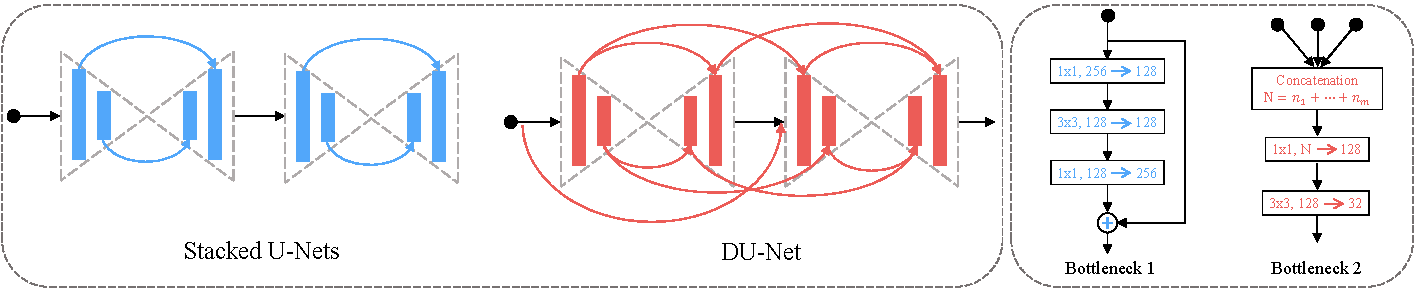
\includegraphics[width=1.0\linewidth]{figures/framework-cropped.pdf}
\caption{Illustration of stacked U-Nets and DU-Net. Stacked U-Nets has skip connections only within each U-Net. In contrast, DU-Net also connects blocks with the same semantic meanings across different U-Nets. The feature reuse could significantly reduce the size of bottleneck in each block, as shown in the right figure. Consequently, with the same number of U-Nets, DU-Net has only 30\% parameters of stacked U-Nets.}
\label{fig:framework}
\end{figure*}

% 
Our solution to those efficiency issues is threefold. {\bf First}, instead of connecting all stacked U-Nets, we only connect a U-Net to its $K$ successors. We name it as the $order$-$K$ connectivity, which aims to balance the fitting accuracy and parameter efficiency by cutting off long-distance connections. {\bf Second}, we employ a memory-efficient implementation in training. The key idea is to reuse a pre-allocated memory so all connected blocks could share the same memory. Compared with the naive implementation, this strategy makes it possible to train a very deep DU-Net (actually, $2\times$ deeper). {\bf Third}, to further improve the efficiency, we investigate an iterative design that may reduce the model size to one half. More specifically, the output of the first pass of the DU-Net is used as the input of the second pass, where detection or regression loss is applied as supervision. 

% %G%
% In view of deploying our approach on mobile devices, we further attempt to quantize weights, inputs, and gradients of DU-Net to low bit-width discrete values. This not only decreases the high precision operations but also shrinks the memory usage during training. By network quantization, the size of trained model can also be largely compressed.
% %G%
Besides shrinking the number of network parameters, we also study to further quantize each parameter. This motivates from the ubiquitous mobile applications. Although current mobile devices could carry models of dozens of MBs, deploying such networks requires high-end GPUs. However, quantized models could be accelerated by some specifically designed low-cost hardwares. Beyond only deploying models on mobile devices \cite{li2017deeprebirth}, training deep neural networks on distributed mobile devices emerges recently \cite{mcmahan2016communication}. To this end, we also try to quantize not only the model parameters but also its inputs (intermediate features) and gradients in training. This is the first attempt to investigate training landmark localizers using quantized inputs and gradients.


In summary, our key contributions are:
\begin{itemize}
    \item To the best of our knowledge, we are the first to propose quantized densely connected U-Nets for visual landmark localization, which largely improves the information flow and feature reuse at the semantic level.
    \item We propose the $order$-$K$ connectivity to balance accuracy and efficiency. It decreases the growth of model size from quadratic to linear by removing trivial connections. Experiments show it could reduce $\sim$70\% parameters of state-of-the-art landmark localizers.
    \item Very deep U-Nets can be trained using a memory-efficient implementation, where pre-allocated memory is reused by all connected blocks.
    \item We further investigate an iterative refinement that may cut down half of the model size, by forwarding DU-Net twice using either detection or regression supervision.
    %G%
    \item Different from previous efforts of quantizing only the model parameters, we are the first to quantize their inputs and gradients for better training efficiency on landmark localization tasks. By choosing appropriate quantization bit-widths for weights, inputs and gradients, quantized DU-Net achieves $\sim$75\% training memory saving with comparable performance. 
    %G%
    \item Exhaustive experiments are performed to validate DU-Net in different aspects. In both human pose estimation and face alignment, DU-Net demonstrates comparable localization accuracy and use $\sim$2\% model size compared with state-of-the-art methods.
\end{itemize}

% We are the first to deploy network quantization for better training efficiency on localization tasks. By choosing appropriate quantization bit-widths for weights, inputs and gradients, quantized DU-Net achieves at least 32$\times$ memory saving with comparable performance to the-state-of-art approaches. 


%The landmark localization such as human pose estimation \cite{toshev2014deeppose,newell2016stacked,wei2016convolutional}, facial landmark localization \cite{xiong2013supervised,zhang2014facial,sagonas2013300}, etc, plays an important role in the higher-level image understanding. The Convolutional Neural Networks (CNNs) have dominated this field, among which recent architecture of stacked hourglasses \cite{newell2016stacked}, a variant of the U-Net \cite{ronneberger2015unet}, becomes a standard solution. The skip connections between top-down and bottom-up blocks within a U-Net could preserve the spatial information and increase the gradient flow. With multiple U-Nets stacked together, the prediction could be refined stage by stage. However, the connections are only within each U-Net of the stacked hourglasses and no explicit connections exist between U-Nets, which may impede the information flow across them. And the blocks with the same semantics in different U-Nets cannot share features, leading to many redundant parameters. 

% Its success attributes to three key factors: repeated top-down, bottom-up inferences, intermediate supervisions and residual bottlenecks \cite{}. 

% The multiple stage top-down and bottom-up processing could better integrate both the local and global visual contexts into the final prediction. The intermediate supervision and residual bottlenecks, on the other hand, could alleviate the gradient vanish problem in deep networks.
%In this paper, we propose to densely connect stacked U-Nets by linking blocks with the same semantics in different U-Nets. We refer to this architecture as {\it Dense U-Nets}. The blocks in a U-Net could get direct inputs from its connected blocks in all preceding U-Nets, making the information flow more efficiently among the U-Nets. The feature reuse at each resolution could reduce the parameters in each block. The dense connectivity in our Dense U-Nets is different from that of DenseNet \cite{huang2016densely}. More specifically, layers only within each single block of the DenseNet are connected. In contrast, we connect blocks lying across the whole Dense U-Nets and connections of hierarchical blocks are mixed together. An illustration is given in Figure \ref{fig:framework}. We name it as the {\it global dense connectivity} to differentiate from the local one in the DenseNet.

% Besides, features in the Dense U-Nets are fused by the concatenation which could facilitate the information flow compared with the summation operation in the stacked hourglasses.

% Although the dense connectivity in our Dense U-Nets is similar with that of DenseNet \cite{}, 
% More recently, the DenseNet \cite{} achieves superior image classification performance over the ResNet \cite{} in terms of both the accuracy and model size, which benefits from the dense connections between layers. Its key insight is the feature reuse between layers of the same resolutions. The dense connectivity in the DenseNet, existing within one block, is local. By extending this principle, we propose a global dense connectivity, in contrast to the local connectivity in \cite{}, that blocks at the same locations of different U-Nets are connected. Hence, we refer to this architecture as {\it Dense U-Nets}. To our best knowledge, we are the first to generalize the local dense connectivity into the stacked U-Nets. 
% The global dense connectivity could make it easier to train much deeper stacked U-Nets.

% This motivates us to replace the residual modules  in the stacked hourglasses with the dense connected layers. However, this dense connectivity exists only locally within a contiguous  block in which all feature maps have the same spatial resolution. A U-Net, on the other hand, consists of a sequence of top-down and bottom-up blocks. A straight way is to turn each block into a dense block with multiple layers. However, this would sacrifice the spirit of stacked hourglasses that multiple stacked hourglasses outperform a single hourglass with multiple layers in each block.

% In order to integrate the structure of stacked U-Nets together with the idea of dense connectivity, we propose a global dense connectivity, in contrast to the local connectivity in \cite{}, that blocks at the same locations of different U-Nets are connected. Hence, we refer to this architecture as {\it Dense U-Nets}. The connected layers in the Dense U-Nets distribute along the whole network rather than in local continuous blocks. Compared with the local residual modules in the stacked hourglasses, the global dense connections could significantly facilitate the gradient to flow across stacked U-Nets.

%In practice, the Dense U-Nets have the efficiency problems of both parameter and training memory. First, suppose a Dense U-Nets contains $n$ U-Nets, there would be $O(n(n-1)/2)$ connections. Even though we use the dense bottleneck in Figure \ref{fig:framework}, the number of conv($1\times 1$) parameters still has the quadratic growth. Inspired from the Variable Order Markov (VOM) models \cite{begleiter2004prediction}, we propose the order-K connectivity that, instead of linking all the U-Nets, we connect only a fixed number of U-Nets. The goal is to use the minimum connections achieving the most obvious improvements. The multiple intermediate supervisions in the Dense U-Nets are good compensates for the order-K connectivity since they could provide additional gradients. The DenseNet does not have this advantage since it has only one supervision at the end.

% Furthermore, different from the DenseNet with only one supervision, the Dense U-Nets have multiple intermediate supervisions. The global dense connections plus the intermediate supervisions could bring faster convergence on the training set, but also gives rise to the concern of overfitting. Inspired from the Variable Order Markov (VOM) models \cite{}, we propose the order-K connectivity that, instead of linking all the U-Nets, we connect only a fixed number of U-Nets. The goal is to use the minimum connections achieving the most obvious improvement. Another advantage of order-K connectivity is that it has fewer parameters compared with the dense connectivity.

%Benefiting from the order-K connectivity, the Dense U-Nets could achieve comparable performance of stacked hourglasses with only one-third parameters. However, a naive implementation of the order-K connectivity could make the training very memory expensive. Therefore, we employ the memory efficient implementation \cite{pleiss2017memory}. The key idea is to share memories for time efficient operations such as concatenation and batch norm \cite{ioffe2015batch} within the connected layers. By pre-allocating a fixed memory, the later features produced by these operations would replace earlier features. So we need to re-compute those replaced features in the backward phase. The memory efficient implementation makes it possible to train Dense U-Nets two times deeper than the stacked hourglasses. 

%Furthermore, we also investigate to use the iterative refinement improving the parameter efficiency. Given a Dense U-Nets, we compare its performance with another Dense U-Nets with only half depth but an additional iteration. Besides, both detection and regression losses \cite{bulat2016human} were used in the landmark detection tasks, but there is no investigation yet about how they independently and collaboratively affect the prediction. We will give their detailed comparison in our experiments.

%In summary, the key contributions are:
%\begin{itemize}
%    \item To our best knowledge, we are the first to use the dense connectivity among the stacked U-Nets. The global dense connectivity in our Dense U-Nets is different from the local one in the DenseNet \cite{huang2016densely}.
%    \item We propose the order-K connectivity to make the Dense U-Nets parameter efficient. The order-K connectivity could decrease the growth of conv($1\times 1$) parameters from quadratic to linear. With comparable performance as the stacked hourglasses \cite{newell2016stacked}, it makes the Dense U-Nets require only one-third parameters. 
%    \item The memory efficient implementation of Dense U-Nets is provided to reduce its training memory usage. It makes it possible to train Dense U-Nets two times deeper than the stacked hourglasses.
%    \item We further explore using iterative refinement to improvement the parameter efficiency. At the same time, we investigate how different combinations of the detection and regression losses affect the performance.
%\end{itemize}

\section{Background}

The goal of reducing sequential computation also forms the foundation of the Extended Neural GPU \citep{extendedngpu}, ByteNet \citep{NalBytenet2017} and ConvS2S \citep{JonasFaceNet2017}, all of which use convolutional neural networks as basic building block, computing hidden representations in parallel for all input and output positions. In these models, the number of operations required to relate signals from two arbitrary input or output positions grows in the distance between positions, linearly for ConvS2S and logarithmically for ByteNet. This makes it more difficult to learn dependencies between distant positions \citep{hochreiter2001gradient}. In the Transformer this is reduced to a constant number of operations, albeit at the cost of reduced effective resolution due to averaging attention-weighted positions, an effect we counteract with Multi-Head Attention as described in section~\ref{sec:attention}. 

Self-attention, sometimes called intra-attention is an attention mechanism relating different positions of a single sequence in order to compute a representation of the sequence. Self-attention has been used successfully in a variety of tasks including reading comprehension, abstractive summarization, textual entailment and learning task-independent sentence representations \citep{cheng2016long, decomposableAttnModel, paulus2017deep, lin2017structured}.

End-to-end memory networks are based on a recurrent attention mechanism instead of sequence-aligned recurrence and have been shown to perform well on simple-language question answering and language modeling tasks \citep{sukhbaatar2015}.

To the best of our knowledge, however, the Transformer is the first transduction model relying entirely on self-attention to compute representations of its input and output without using sequence-aligned RNNs or convolution.
In the following sections, we will describe the Transformer, motivate self-attention and discuss its advantages over models such as \citep{neural_gpu, NalBytenet2017} and \citep{JonasFaceNet2017}.


%\citep{JonasFaceNet2017} report new SOTA on machine translation for English-to-German (EnDe), Enlish-to-French (EnFr) and English-to-Romanian language pairs. 

%For example,! in MT, we must draw information from both input and previous output words to translate an output word accurately. An attention layer \citep{bahdanau2014neural} can connect a very large number of positions at low computation cost, making it an essential ingredient in competitive recurrent models for machine translation.

%A natural question to ask then is, "Could we replace recurrence with attention?". \marginpar{Don't know if it's the most natural question to ask given the previous statements. Also, need to say that the complexity table summarizes these statements} Such a model would be blessed with the computational efficiency of attention and the power of cross-positional communication. In this work, show that pure attention models work remarkably well for MT, achieving new SOTA results on EnDe and EnFr, and can be trained in under $2$ days on xyz architecture. 

%After the seminal models introduced in \citep{sutskever14, bahdanau2014neural, cho2014learning}, recurrent models have become the dominant solution for both sequence modeling and sequence-to-sequence transduction. Many efforts such as \citep{wu2016google,luong2015effective,jozefowicz2016exploring} have pushed the boundaries of machine translation (MT) and language modeling with recurrent endoder-decoder and recurrent language models. Recent effort \citep{shazeer2017outrageously} has successfully combined the power of conditional computation with sequence models to train very large models for MT, pushing SOTA at lower computational cost.

%Recurrent models compute a vector of hidden states $h_t$, for each time step $t$ of computation. $h_t$ is a function of both the input at time $t$ and the previous hidden state $h_t$. This dependence on the previous hidden state precludes processing all timesteps at once, instead requiring long sequences of sequential operations.  In practice, this results in greatly reduced computational efficiency, as on modern computing hardware, a single operation on a large batch is much faster than a large number of operations on small batches.  The problem gets worse at longer sequence lengths. Although sequential computation is not a severe bottleneck at inference time, as autoregressively generating each output requires all previous outputs, the inability to compute scores at all output positions at once hinders us from rapidly training our models over large datasets. Although impressive work such as \citep{Kuchaiev2017Factorization} is able to significantly accelerate the training of LSTMs with factorization tricks, we are still bound by the linear dependence on sequence length.

%If the model could compute hidden states at each time step using only the inputs and outputs,  it would be liberated from the dependence on results from previous time steps during training. This line of thought is the foundation of recent efforts such as the Markovian neural GPU \citep{neural_gpu}, ByteNet \citep{NalBytenet2017} and ConvS2S \citep{JonasFaceNet2017}, all of which use convolutional neural networks as a building block to compute hidden representations simultaneously for all timesteps, resulting in $O(1)$ sequential time complexity. \citep{JonasFaceNet2017} report new SOTA on machine translation for English-to-German (EnDe), Enlish-to-French (EnFr) and English-to-Romanian language pairs. 

%A crucial component for accurate sequence prediction is modeling cross-positional communication. For example, in MT, we must draw information from both input and previous output words to translate an output word accurately. An attention layer \citep{bahdanau2014neural} can connect a very large number of positions at a low computation cost, also $O(1)$ sequential time complexity, making it an essential ingredient in recurrent encoder-decoder architectures for MT. A natural question to ask then is, "Could we replace recurrence with attention?". \marginpar{Don't know if it's the most natural question to ask given the previous statements. Also, need to say that the complexity table summarizes these statements} Such a model would be blessed with the computational efficiency of attention and the power of cross-positional communication. In this work, show that pure attention models work remarkably well for MT, achieving new SOTA results on EnDe and EnFr, and can be trained in under $2$ days on xyz architecture. 



%Note: Facebook model is no better than RNNs in this regard, since it requires a number of layers proportional to the distance you want to communicate.  Bytenet is more promising, since it requires a logarithmnic number of layers (does bytenet have SOTA results)?   

%Note: An attention  layer can connect a very large number of positions at a low computation cost in O(1) sequential operations.  This is why encoder-decoder attention has been so successful in seq-to-seq models so far.  It is only natural, then, to also use attention to connect the timesteps of the same sequence.

%Note: I wouldn't say that long sequences are not a problem during inference.  It would be great if we could infer with no long sequences.  We could just say later on that, while our training graph is constant-depth, our model still requires sequential operations in the decoder part during inference due to the autoregressive nature of the model.   

%\begin{table}[h!]
%\caption{Attention models are quite efficient for cross-positional communications when sequence length is smaller than channel depth. $n$ represents the sequence length and $d$ represents the channel depth.}
%\label{tab:op_complexities}
%\begin{center}
%\vspace{-5pt}
%\scalebox{0.75}{

%\begin{tabular}{l|c|c|c}
%\hline \hline
%Layer Type & Receptive & Complexity & Sequential  \\
%           & Field     &            & Operations  \\
%\hline
%Pointwise Feed-Forward & $1$ & $O(n \cdot d^2)$ & $O(1)$ \\
%\hline
%Recurrent & $n$ & $O(n \cdot d^2)$ & $O(n)$ \\
%\hline
%Convolutional & $r$ & $O(r \cdot n \cdot d^2)$ & $O(1)$ \\
%\hline
%Convolutional (separable) & $r$ & $O(r \cdot n \cdot d + n %\cdot d^2)$ & $O(1)$ \\
%\hline
%Attention & $r$ & $O(r \cdot n \cdot d)$ & $O(1)$ \\
%\hline \hline
%\end{tabular}
%}
%\end{center}
%\end{table}

\section{Model Architecture}

\begin{figure}
  \centering
  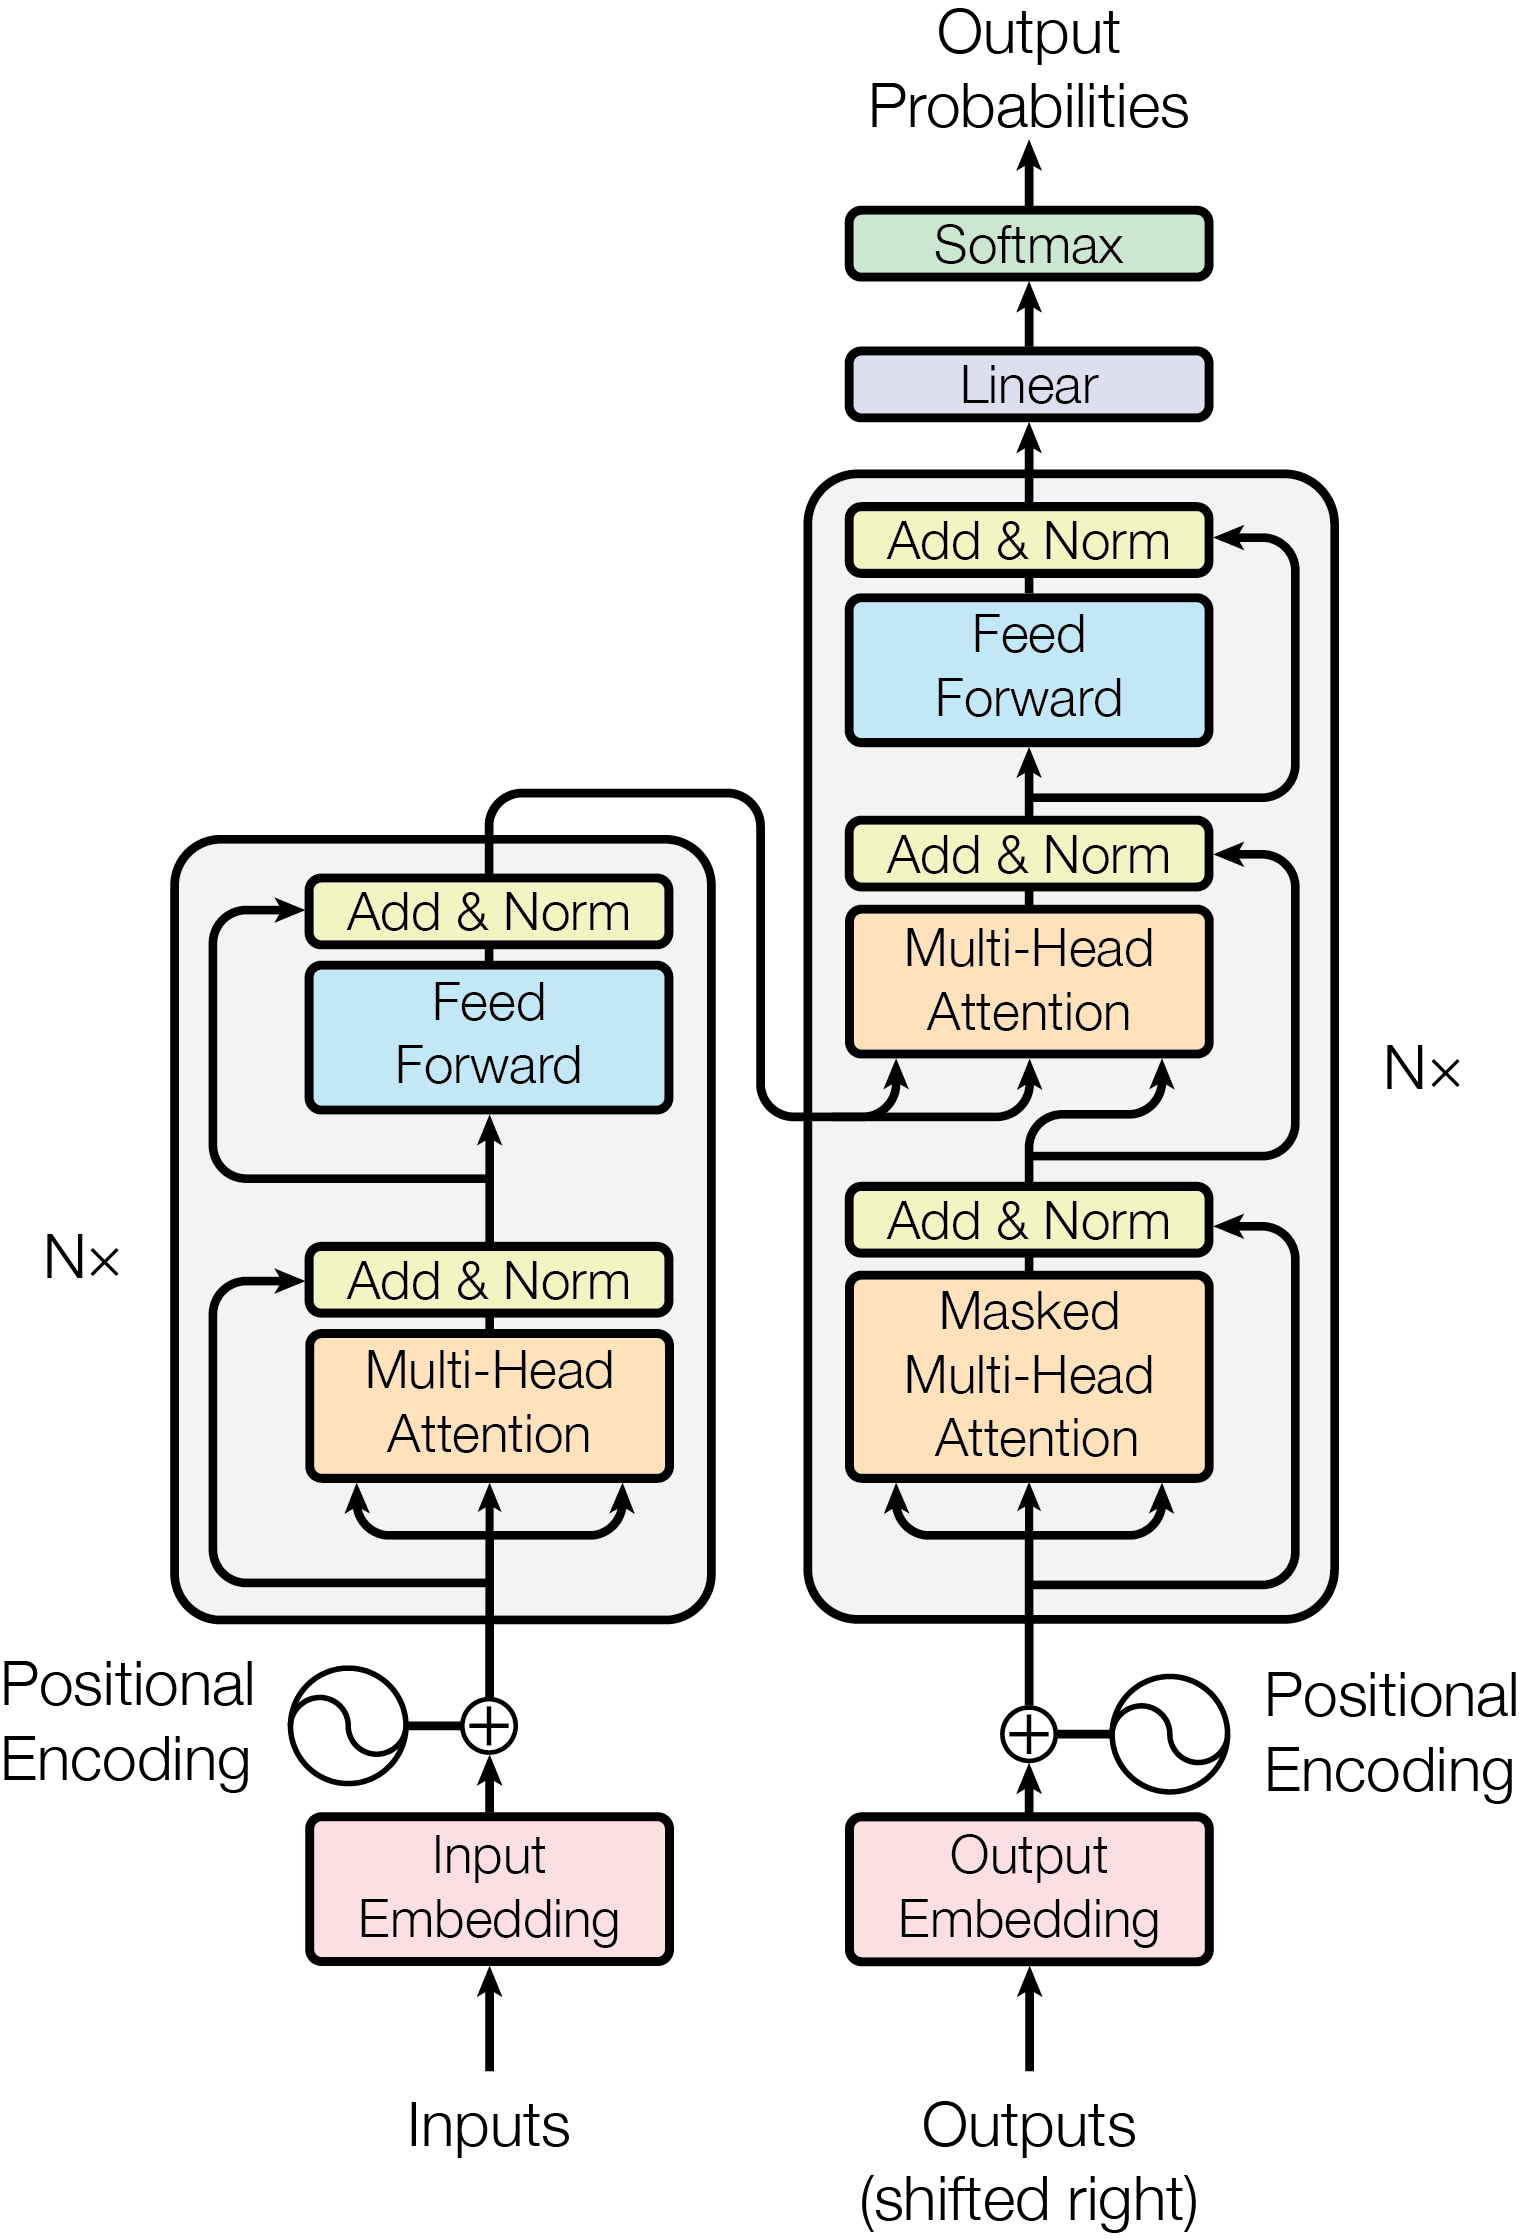
\includegraphics[scale=0.6]{Figures/ModalNet-21}
  \caption{The Transformer - model architecture.}
  \label{fig:model-arch}
\end{figure}

% Although the primary workhorse of our model is attention, 
%Our model maintains the encoder-decoder structure that is common to many so-called sequence-to-sequence models \citep{bahdanau2014neural,sutskever14}.  As in all such architectures, the encoder computes a representation of the input sequence, and the decoder consumes these representations along with the output tokens to autoregressively produce the output sequence.  Where, traditionally, the encoder and decoder contain stacks of recurrent or convolutional layers, our encoder and decoder stacks are composed of attention layers and position-wise feed-forward layers (Figure~\ref{fig:model-arch}).  The following sections describe the gross architecture and these particular components in detail.

Most competitive neural sequence transduction models have an encoder-decoder structure \citep{cho2014learning,bahdanau2014neural,sutskever14}. Here, the encoder maps an input sequence of symbol representations $(x_1, ..., x_n)$ to a sequence of continuous representations $\mathbf{z} = (z_1, ..., z_n)$. Given $\mathbf{z}$, the decoder then generates an output sequence $(y_1,...,y_m)$ of symbols one element at a time. At each step the model is auto-regressive \citep{graves2013generating}, consuming the previously generated symbols as additional input when generating the next.

The Transformer follows this overall architecture using stacked self-attention and point-wise, fully connected layers for both the encoder and decoder, shown in the left and right halves of Figure~\ref{fig:model-arch}, respectively.

\subsection{Encoder and Decoder Stacks}

\paragraph{Encoder:}The encoder is composed of a stack of $N=6$ identical layers. Each layer has two sub-layers. The first is a multi-head self-attention mechanism, and the second is a simple, position-wise fully connected feed-forward network.   We employ a residual connection \citep{he2016deep} around each of the two sub-layers, followed by layer normalization \cite{layernorm2016}.  That is, the output of each sub-layer is $\mathrm{LayerNorm}(x + \mathrm{Sublayer}(x))$, where $\mathrm{Sublayer}(x)$ is the function implemented by the sub-layer itself.  To facilitate these residual connections, all sub-layers in the model, as well as the embedding layers, produce outputs of dimension $\dmodel=512$.

\paragraph{Decoder:}The decoder is also composed of a stack of $N=6$ identical layers.  In addition to the two sub-layers in each encoder layer, the decoder inserts a third sub-layer, which performs multi-head attention over the output of the encoder stack.  Similar to the encoder, we employ residual connections around each of the sub-layers, followed by layer normalization.  We also modify the self-attention sub-layer in the decoder stack to prevent positions from attending to subsequent positions.  This masking, combined with fact that the output embeddings are offset by one position, ensures that the predictions for position $i$ can depend only on the known outputs at positions less than $i$.

% In our model (Figure~\ref{fig:model-arch}), the encoder and decoder are composed of stacks of alternating self-attention layers (for cross-positional communication) and position-wise feed-forward layers (for in-place computation).  In addition, the decoder stack contains encoder-decoder attention layers.  Since attention is agnostic to the distances between words, our model requires a "positional encoding" to be added to the encoder and decoder input. The following sections describe all of these components in detail.

\subsection{Attention} \label{sec:attention}
An attention function can be described as mapping a query and a set of key-value pairs to an output, where the query, keys, values, and output are all vectors.  The output is computed as a weighted sum of the values, where the weight assigned to each value is computed by a compatibility function of the query with the corresponding key.

\subsubsection{Scaled Dot-Product Attention} \label{sec:scaled-dot-prod}

% \begin{figure}
%   \centering
%   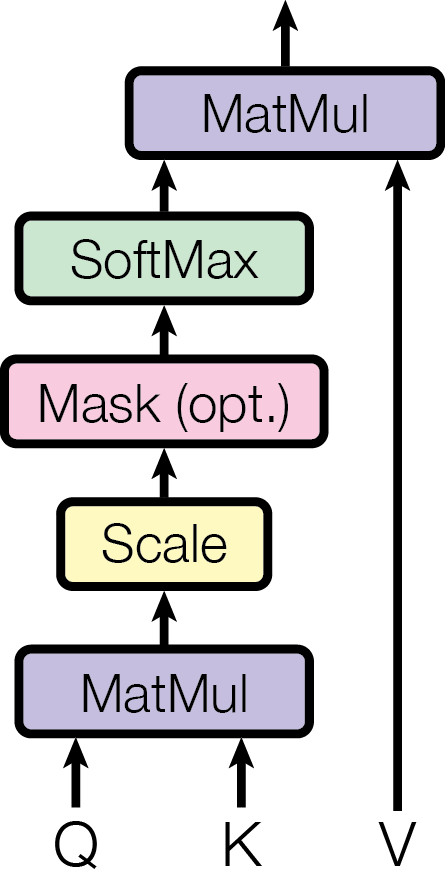
\includegraphics[scale=0.6]{Figures/ModalNet-19}
%   \caption{Scaled Dot-Product Attention.}
%   \label{fig:multi-head-att}
% \end{figure}

We call our particular attention "Scaled Dot-Product Attention" (Figure~\ref{fig:multi-head-att}).   The input consists of queries and keys of dimension $d_k$, and values of dimension $d_v$.  We compute the dot products of the query with all keys, divide each by $\sqrt{d_k}$, and apply a softmax function to obtain the weights on the values.

In practice, we compute the attention function on a set of queries simultaneously, packed together into a matrix $Q$.   The keys and values are also packed together into matrices $K$ and $V$.  We compute the matrix of outputs as:

\begin{equation}
   \mathrm{Attention}(Q, K, V) = \mathrm{softmax}(\frac{QK^T}{\sqrt{d_k}})V
\end{equation}

The two most commonly used attention functions are additive attention \citep{bahdanau2014neural}, and dot-product (multiplicative) attention.  Dot-product attention is identical to our algorithm, except for the scaling factor of $\frac{1}{\sqrt{d_k}}$. Additive attention computes the compatibility function using a feed-forward network with a single hidden layer.  While the two are similar in theoretical complexity, dot-product attention is much faster and more space-efficient in practice, since it can be implemented using highly optimized matrix multiplication code. 

%We scale the dot products by $1/\sqrt{d_k}$ to limit the magnitude of the dot products, which works well in practice. Otherwise, we found applying the softmax to often result in weights very close to 0 or 1, and hence minuscule gradients.

% Already described in the subsequent section
%When used as part of decoder self-attention, an optional mask function is applied just before the softmax to prevent positions from attending to subsequent positions.   This mask simply sets the logits corresponding to all illegal connections (those outside of the lower triangle) to $-\infty$.

%\paragraph{Comparison to Additive Attention: } We choose dot product attention over additive attention \citep{bahdanau2014neural} since it can be computed using highly optimized matrix multiplication code.  This optimization is particularly important to us, as we employ many attention layers in our model.

While for small values of $d_k$ the two mechanisms perform similarly, additive attention outperforms dot product attention without scaling for larger values of $d_k$ \citep{DBLP:journals/corr/BritzGLL17}. We suspect that for large values of $d_k$, the dot products grow large in magnitude, pushing the softmax function into regions where it has extremely small gradients  \footnote{To illustrate why the dot products get large, assume that the components of $q$ and $k$ are independent random variables with mean $0$ and variance $1$.  Then their dot product, $q \cdot k = \sum_{i=1}^{d_k} q_ik_i$, has mean $0$ and variance $d_k$.}. To counteract this effect, we scale the dot products by $\frac{1}{\sqrt{d_k}}$.


%We suspect this to be caused by the dot products growing too large in magnitude to result in useful gradients after applying the softmax function.  To counteract this, we scale the dot product by $1/\sqrt{d_k}$.


\subsubsection{Multi-Head Attention} \label{sec:multihead}

\begin{figure}
\begin{minipage}[t]{0.5\textwidth}
  \centering
  Scaled Dot-Product Attention \\
  \vspace{0.5cm}
  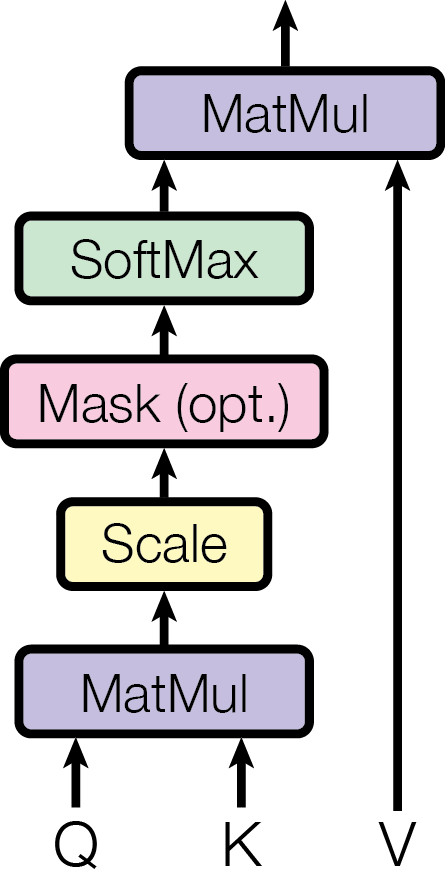
\includegraphics[scale=0.6]{Figures/ModalNet-19}
\end{minipage}
\begin{minipage}[t]{0.5\textwidth}
  \centering 
  Multi-Head Attention \\
  \vspace{0.1cm}
  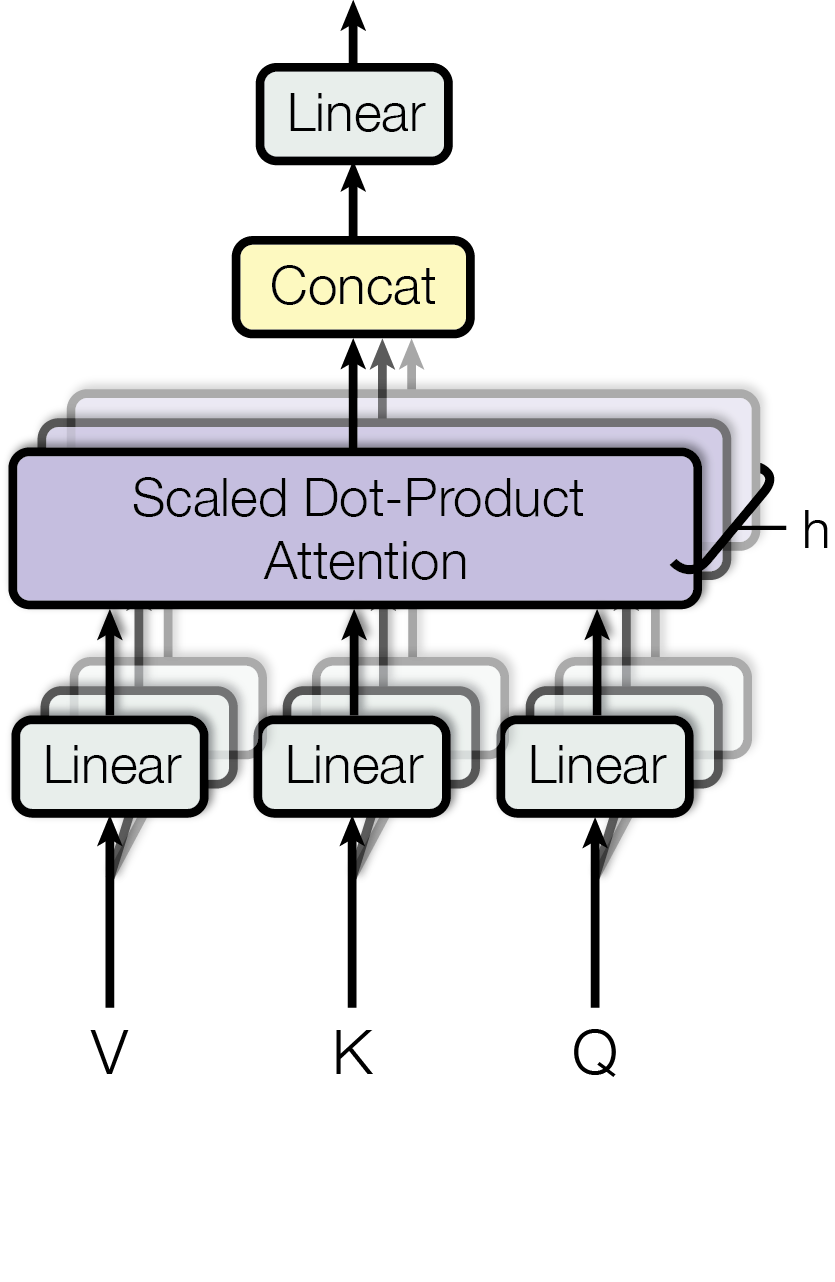
\includegraphics[scale=0.6]{Figures/ModalNet-20}  
\end{minipage}


  % \centering

  \caption{(left) Scaled Dot-Product Attention. (right) Multi-Head Attention consists of several attention layers running in parallel.}
  \label{fig:multi-head-att}
\end{figure}

Instead of performing a single attention function with $\dmodel$-dimensional keys, values and queries, we found it beneficial to linearly project the queries, keys and values $h$ times with different, learned linear projections to $d_k$, $d_k$ and $d_v$ dimensions, respectively.
On each of these projected versions of queries, keys and values we then perform the attention function in parallel, yielding $d_v$-dimensional output values. These are concatenated and once again projected, resulting in the final values, as depicted in Figure~\ref{fig:multi-head-att}.

Multi-head attention allows the model to jointly attend to information from different representation subspaces at different positions. With a single attention head, averaging inhibits this.

\begin{align*}
    \mathrm{MultiHead}(Q, K, V) &= \mathrm{Concat}(\mathrm{head_1}, ..., \mathrm{head_h})W^O\\
%    \mathrm{where} \mathrm{head_i} &= \mathrm{Attention}(QW_Q_i^{\dmodel \times d_q}, KW_K_i^{\dmodel \times d_k}, VW^V_i^{\dmodel \times d_v})\\
    \text{where}~\mathrm{head_i} &= \mathrm{Attention}(QW^Q_i, KW^K_i, VW^V_i)\\
\end{align*}

Where the projections are parameter matrices $W^Q_i \in \mathbb{R}^{\dmodel \times d_k}$, $W^K_i \in \mathbb{R}^{\dmodel \times d_k}$, $W^V_i \in \mathbb{R}^{\dmodel \times d_v}$ and $W^O \in \mathbb{R}^{hd_v \times \dmodel}$.


%find it better (and no more expensive) to have multiple parallel attention layers (each over the full set of positions) with proportionally lower-dimensional keys, values and queries.  We call this "Multi-Head Attention" (Figure~\ref{fig:multi-head-att}).  The keys, values, and queries for each of these parallel attention layers are computed by learned linear transformations of the inputs to the multi-head attention.  We use different linear transformations across different parallel attention layers.  The output of the parallel attention layers are concatenated, and then passed through a final learned linear transformation. 

In this work we employ $h=8$ parallel attention layers, or heads. For each of these we use $d_k=d_v=\dmodel/h=64$.
Due to the reduced dimension of each head, the total computational cost is similar to that of single-head attention with full dimensionality.

\subsubsection{Applications of Attention in our Model}

The Transformer uses multi-head attention in three different ways: 
\begin{itemize}
 \item In "encoder-decoder attention" layers, the queries come from the previous decoder layer, and the memory keys and values come from the output of the encoder.   This allows every position in the decoder to attend over all positions in the input sequence.  This mimics the typical encoder-decoder attention mechanisms in sequence-to-sequence models such as \citep{wu2016google, bahdanau2014neural,JonasFaceNet2017}.

 \item The encoder contains self-attention layers.  In a self-attention layer all of the keys, values and queries come from the same place, in this case, the output of the previous layer in the encoder.   Each position in the encoder can attend to all positions in the previous layer of the encoder.

 \item Similarly, self-attention layers in the decoder allow each position in the decoder to attend to all positions in the decoder up to and including that position.  We need to prevent leftward information flow in the decoder to preserve the auto-regressive property.  We implement this inside of scaled dot-product attention by masking out (setting to $-\infty$) all values in the input of the softmax which correspond to illegal connections.  See Figure~\ref{fig:multi-head-att}.

\end{itemize}

\subsection{Position-wise Feed-Forward Networks}\label{sec:ffn}

In addition to attention sub-layers, each of the layers in our encoder and decoder contains a fully connected feed-forward network, which is applied to each position separately and identically.  This consists of two linear transformations with a ReLU activation in between.

\begin{equation}
   \mathrm{FFN}(x)=\max(0, xW_1 + b_1) W_2 + b_2
\end{equation}

While the linear transformations are the same across different positions, they use different parameters from layer to layer. Another way of describing this is as two convolutions with kernel size 1.  The dimensionality of input and output is $\dmodel=512$, and the inner-layer has dimensionality $d_{ff}=2048$.



%In the appendix, we describe how the position-wise feed-forward network can also be seen as a form of attention.

%from Jakob: The number of operations required for the model to relate signals from two arbitrary input or output positions grows in the distance between positions in input or output, linearly for ConvS2S and logarithmically for ByteNet, making it harder to learn dependencies between these positions \citep{hochreiter2001gradient}. In the transformer this is reduced to a constant number of operations, albeit at the cost of effective resolution caused by averaging attention-weighted positions, an effect we aim to counteract with multi-headed attention.


%Figure~\ref{fig:simple-att} presents a simple attention function, $A$, with a single head, that forms the basis of our multi-head attention. $A$ takes a query key vector $\kq$, matrices of memory keys $\km$ and memory values $\vm$ ,and produces a query value vector $\vq$ as 
%\begin{equation*} \label{eq:attention}
%    A(\kq, \km, \vm) = {\vm}^T (Softmax(\km \kq).
%\end{equation*}
%We linearly transform $\kq,\,\km$, and $\vm$ with learned matrices ${\Wkq \text{,} \, \Wkm}$, and ${\Wvm}$ before calling the attention function, and transform the output query with $\Wvq$ before handing it to the feed forward layer. Each attention layer has it's own set of transformation matrices, which are shared across all query positions. $A$ is applied in parallel for each query position, and is implemented very efficiently as a batch of matrix multiplies. The self-attention and encoder-decoder attention layers use $A$, but with different arguments. For example, in encdoder self-attention, queries in encoder layer $i$ attention to memories in encoder layer $i-1$. To ensure that decoder self-attention layers do not look at future words, we add $- \inf$ to the softmax logits in positions $j+1$ to query length for query position $l$.  

%In simple attention, the query value is a weighted combination of the memory values where the attention weights sum to one. Although this function performs well in practice, the constraint on attention weights can restrict the amount of information that flows from memories to queries because the query cannot focus on multiple memory positions at once, which might be desirable when translating long sequences. \marginpar{@usz, could you think of an example of this ?} We remedy this by maintaining multiple attention heads at each query position that attend to all memory positions in parallel, with a different set of parameters  per attention head $h$. 
%\marginpar{}

\subsection{Embeddings and Softmax}
Similarly to other sequence transduction models, we use learned embeddings to convert the input tokens and output tokens to vectors of dimension $\dmodel$.  We also use the usual learned linear transformation and softmax function to convert the decoder output to predicted next-token probabilities.  In our model, we share the same weight matrix between the two embedding layers and the pre-softmax linear transformation, similar to \citep{press2016using}.   In the embedding layers, we multiply those weights by $\sqrt{\dmodel}$.


\subsection{Positional Encoding}
Since our model contains no recurrence and no convolution, in order for the model to make use of the order of the sequence, we must inject some information about the relative or absolute position of the tokens in the sequence.  To this end, we add "positional encodings" to the input embeddings at the bottoms of the encoder and decoder stacks.  The positional encodings have the same dimension $\dmodel$ as the embeddings, so that the two can be summed.   There are many choices of positional encodings, learned and fixed \citep{JonasFaceNet2017}.

In this work, we use sine and cosine functions of different frequencies:

\begin{align*}
    PE_{(pos,2i)} = sin(pos / 10000^{2i/\dmodel}) \\
    PE_{(pos,2i+1)} = cos(pos / 10000^{2i/\dmodel})
\end{align*}

where $pos$ is the position and $i$ is the dimension.  That is, each dimension of the positional encoding corresponds to a sinusoid.  The wavelengths form a geometric progression from $2\pi$ to $10000 \cdot 2\pi$.  We chose this function because we hypothesized it would allow the model to easily learn to attend by relative positions, since for any fixed offset $k$, $PE_{pos+k}$ can be represented as a linear function of $PE_{pos}$.

We also experimented with using learned positional embeddings \citep{JonasFaceNet2017} instead, and found that the two versions produced nearly identical results (see Table~\ref{tab:variations} row (E)).  We chose the sinusoidal version because it may allow the model to extrapolate to sequence lengths longer than the ones encountered during training.

 
\section{Why Self-Attention}
%We focus on the general task of mapping one variable-length sequence of symbol representations ${x_1, ..., x_n} \in \mathbb{R}^d$ to another sequence of the same length ${y_1, ..., y_n} \in \mathbb{R}^d$. \marginpar{should we use this notation? alternatively we can just say "d-dimensional vectors"}

In this section we compare various aspects of self-attention layers to the recurrent and convolutional layers commonly used for mapping one variable-length sequence of symbol representations $(x_1, ..., x_n)$ to another sequence of equal length $(z_1, ..., z_n)$, with $x_i, z_i \in \mathbb{R}^d$, such as a hidden layer in a typical sequence transduction encoder or decoder. Motivating our use of self-attention we consider three desiderata.

One is the total computational complexity per layer.
Another is the amount of computation that can be parallelized, as measured by the minimum number of sequential operations required.

The third is the path length between long-range dependencies in the network. Learning long-range dependencies is a key challenge in many sequence transduction tasks. One key factor affecting the ability to learn such dependencies is the length of the paths forward and backward signals have to traverse in the network. The shorter these paths between any combination of positions in the input and output sequences, the easier it is to learn long-range dependencies \citep{hochreiter2001gradient}. Hence we also compare the maximum path length between any two input and output positions in networks composed of the different layer types.

%\subsection{Computational Performance and Path Lengths}

\begin{table}[t]
\caption{
  Maximum path lengths, per-layer complexity and minimum number of sequential operations for different layer types. $n$ is the sequence length, $d$ is the representation dimension, $k$ is the kernel size of convolutions and $r$ the size of the neighborhood in restricted self-attention.}
  %Attention models are quite efficient for cross-positional communications when sequence length is smaller than channel depth.
\label{tab:op_complexities}
\begin{center}
\vspace{-1mm}
%\scalebox{0.75}{

\begin{tabular}{lccc}
\toprule
Layer Type & Complexity per Layer & Sequential & Maximum Path Length  \\
           &             & Operations &   \\
\hline
\rule{0pt}{2.0ex}Self-Attention & $O(n^2 \cdot d)$ & $O(1)$ & $O(1)$ \\
Recurrent & $O(n \cdot d^2)$ & $O(n)$ & $O(n)$ \\

Convolutional & $O(k \cdot n \cdot d^2)$ & $O(1)$ & $O(log_k(n))$ \\
%\cmidrule
Self-Attention (restricted)& $O(r \cdot n \cdot d)$ & $O(1)$ & $O(n/r)$ \\

%Convolutional (separable) & $O(k \cdot n \cdot d + n \cdot d^2)$ & $O(1)$ & $O(log_k(n))$ \\

%Position-wise Feed-Forward & $O(n \cdot d^2)$ & $O(1)$ & $\infty$ \\

%Fully Connected & $O(n^2 \cdot d^2)$ & $O(1)$ & $O(1)$ \\
%Convolutional (separable) & $O(k \cdot n \cdot d + n \cdot d^2)$ & $O(1)$ & $O(log_k(n))$ \\

%Position-wise Feed-Forward & $O(n \cdot d^2)$ & $O(1)$ & $\infty$ \\

%Fully Connected & $O(n^2 \cdot d^2)$ & $O(1)$ & $O(1)$ \\
\bottomrule
\end{tabular}
%}
\end{center}
\end{table}


%\begin{table}[b]
%\caption{
%  Maximum path lengths, per-layer complexity and minimum number of sequential operations for different layer types. $n$ is the sequence length, $d$ is the representation dimensionality, $k$ is the kernel size of convolutions and $r$ the size of the neighborhood in localized self-attention.}
  %Attention models are quite efficient for cross-positional communications when sequence length is smaller than channel depth.
%\label{tab:op_complexities}
%\begin{center}
%\vspace{-1mm}
%%\scalebox{0.75}{
%
%\begin{tabular}{lccc}
%\hline
%Layer Type & Receptive & Complexity per Layer & Sequential  %\\
%           & Field Size     &            & Operations  \\
%\hline
%Self-Attention & $n$ & $O(n^2 \cdot d)$ & $O(1)$ \\
%Recurrent & $n$ & $O(n \cdot d^2)$ & $O(n)$ \\

%Convolutional & $k$ & $O(k \cdot n \cdot d^2)$ & %$O(log_k(n))$ \\
%\hline 
%Self-Attention (localized)& $r$ & $O(r \cdot n \cdot d)$ & %$O(1)$ \\

%Convolutional (separable) & $k$ & $O(k \cdot n \cdot d + n %\cdot d^2)$ & $O(log_k(n))$ \\

%Position-wise Feed-Forward & $1$ & $O(n \cdot d^2)$ & $O(1)$ %\\

%Fully Connected & $n$ & $O(n^2 \cdot d^2)$ & $O(1)$ \\

%\end{tabular}
%%}
%\end{center}
%\end{table}

%The receptive field size of a layer is the number of different input representations that can influence any particular output representation. Recurrent layers and self-attention layers have a full receptive field equal to the sequence length $n$. Convolutional layers have a limited receptive field equal to their kernel width $k$, which is generally chosen to be small in order to limit computational cost.

As noted in Table \ref{tab:op_complexities}, a self-attention layer connects all positions with a constant number of sequentially executed operations, whereas a recurrent layer requires $O(n)$ sequential operations.
In terms of computational complexity, self-attention layers are faster than recurrent layers when the sequence length $n$ is smaller than the representation dimensionality $d$, which is most often the case with sentence representations used by state-of-the-art models in machine translations, such as word-piece \citep{wu2016google} and byte-pair \citep{sennrich2015neural} representations.
To improve computational performance for tasks involving very long sequences, self-attention could be restricted to considering only a neighborhood of size $r$ in the input sequence centered around the respective output position. This would increase the maximum path length to $O(n/r)$. We plan to investigate this approach further in future work.

A single convolutional layer with kernel width $k < n$ does not connect all pairs of input and output positions. Doing so requires a stack of $O(n/k)$ convolutional layers in the case of contiguous kernels, or $O(log_k(n))$ in the case of dilated convolutions \citep{NalBytenet2017}, increasing the length of the longest paths between any two positions in the network.
Convolutional layers are generally more expensive than recurrent layers, by a factor of $k$. Separable convolutions \citep{xception2016}, however, decrease the complexity considerably, to $O(k \cdot n \cdot d + n \cdot d^2)$. Even with $k=n$, however, the complexity of a separable convolution is equal to the combination of a self-attention layer and a point-wise feed-forward layer, the approach we take in our model.

%\subsection{Unfiltered Bottleneck Argument}

%An orthogonal argument can be made for self-attention layers based on when the layer imposes the bottleneck of mapping all of the information used to compute a given output position into a single, fixed-length vector. ...

%There is a second argument for self-attention layers which we call the unfiltered bottleneck argument.   In both recurrent and the convolutional layers, the information that position $i$ receives from the other positions is compressed to a vector of dimension $d$ before it ever can be filtered by the content $x_i$.  More precisely, we can express $y_i = F(i, x_i, G(i, \{x_{j \neq i}\}))$, where $G(i, \{x_{j \neq i}\})$ is a vector of dimension $d$.  Intuitively, we would expect that this would cause a large amount of irrelevant information to crowd out the relevant information.  Self-attention does not suffer from the unfiltered bottleneck problem, since the aggregation happens after filtering, and so, intuitively, we have the chance of transmitting lots of relevant information.

As side benefit, self-attention could yield more interpretable models. We inspect attention distributions from our models and present and discuss examples in the appendix. Not only do individual attention heads clearly learn to perform different tasks, many appear to exhibit behavior related to the syntactic and semantic structure of the sentences.



\section{Training}
This section describes the training regime for our models. 

%In order to speed up experimentation, our ablations are performed relative to a smaller base model described in detail in Section \ref{sec:results}.

\subsection{Training Data and Batching}
We trained on the standard WMT 2014 English-German dataset consisting of about 4.5 million sentence pairs.  Sentences were encoded using byte-pair encoding \citep{DBLP:journals/corr/BritzGLL17}, which has a shared source-target vocabulary of about 37000 tokens. For English-French, we used the significantly larger WMT 2014 English-French dataset consisting of 36M sentences and split tokens into a 32000 word-piece vocabulary \citep{wu2016google}.  Sentence pairs were batched together by approximate sequence length.  Each training batch contained a set of sentence pairs containing approximately 25000 source tokens and 25000 target tokens.  

\subsection{Hardware and Schedule}

We trained our models on one machine with 8 NVIDIA P100 GPUs.  For our base models using the hyperparameters described throughout the paper, each training step took about 0.4 seconds.  We trained the base models for a total of 100,000 steps or 12 hours.  For our big models,(described on the bottom line of table \ref{tab:variations}), step time was 1.0 seconds.  The big models were trained for 300,000 steps (3.5 days).

\subsection{Optimizer} We used the Adam optimizer~\citep{kingma2014adam} with $\beta_1=0.9$, $\beta_2=0.98$ and $\epsilon=10^{-9}$.  We varied the learning rate over the course of training, according to the formula:

\begin{equation}
lrate = \dmodel^{-0.5} \cdot
  \min({step\_num}^{-0.5},
    {step\_num} \cdot {warmup\_steps}^{-1.5})
\end{equation}

This corresponds to increasing the learning rate linearly for the first $warmup\_steps$ training steps, and decreasing it thereafter proportionally to the inverse square root of the step number.  We used $warmup\_steps=4000$.

\subsection{Regularization} \label{sec:reg}

We employ three types of regularization during training: 
\paragraph{Residual Dropout} We apply dropout \citep{srivastava2014dropout} to the output of each sub-layer, before it is added to the sub-layer input and normalized.   In addition, we apply dropout to the sums of the embeddings and the positional encodings in both the encoder and decoder stacks.  For the base model, we use a rate of $P_{drop}=0.1$.

% \paragraph{Attention Dropout} Query to key attentions are structurally similar to hidden-to-hidden weights in a feed-forward network, albeit across positions. The softmax activations yielding attention weights can then be seen as the analogue of hidden layer activations. A natural possibility is to extend dropout \citep{srivastava2014dropout} to attention. We implement attention dropout by dropping out attention weights as,
% \begin{equation*}
%   \mathrm{Attention}(Q, K, V) = \mathrm{dropout}(\mathrm{softmax}(\frac{QK^T}{\sqrt{d}}))V
% \end{equation*}
% In addition to residual dropout, we found attention dropout to be beneficial for our parsing experiments.  

%\paragraph{Symbol Dropout} In the source and target embedding layers, we replace a random subset of the token ids with a sentinel id.  For the base model, we use a rate of $symbol\_dropout\_rate=0.1$.  Note that this applies only to the auto-regressive use of the target ids - not their use in the cross-entropy loss. 

%\paragraph{Attention Dropout} Query to memory attentions are structurally similar to hidden-to-hidden weights in a feed-forward network, albeit across positions. The softmax activations yielding attention weights can then be seen as the analogue of hidden layer activations. A natural possibility is to extend dropout \citep{srivastava2014dropout} to attentions. We implement attention dropout by dropping out attention weights as,
%\begin{equation*}
%   A(Q, K, V) = \mathrm{dropout}(\mathrm{softmax}(\frac{QK^T}{\sqrt{d}}))V
%\end{equation*}
%As a result, the query will not be able to access the memory values at the dropped out position. In our experiments, we tried attention dropout rates of 0.2, and 0.3, and found it to work favorably for English-to-German translation.
%$attention\_dropout\_rate=0.2$.

\paragraph{Label Smoothing} During training, we employed label smoothing of value $\epsilon_{ls}=0.1$ \citep{DBLP:journals/corr/SzegedyVISW15}.  This hurts perplexity, as the model learns to be more unsure, but improves accuracy and BLEU score.

 
\section{Results} \label{sec:results}
\section{Experiments}
\label{sec:results}

In this section we describe the results of many experiments, comparing our Matching Networks model against strong baselines.
All of our experiments revolve around the same basic task: an $N$-way $k$-shot learning task.
Each method is providing with a set of $k$ labelled examples from each of $N$ classes that have not previously been trained upon.
The task is then to classify a disjoint batch of unlabelled examples into one of these $N$ classes.
Thus random performance on this task stands at $1/N$.
We compared a number of alternative models, as baselines, to Matching Networks.

Let $L'$ denote the held-out subset of labels which we only use for one-shot. Unless otherwise specified, training is always on $\neq\!\! L'$, and test in one-shot mode on $L'$.

We ran one-shot experiments on three data sets: two image classification sets (Omniglot \cite{omniglot} and ImageNet \cite[ILSVRC-2012]{ImageNet}) and one language modeling (Penn Treebank).
The experiments on the three data sets comprise a diverse set of qualities in terms of complexity, sizes, and modalities. 

\subsection{Image Classification Results}

\begin{table}[b]\small
\begin{center}
\begin{tabular}{l@{\hskip \colspaceL}l@{\hskip \colspaceL}l@{\hskip \colspaceL}r@{\hskip \colspaceS}r@{\hskip \colspaceL}r@{\hskip \colspaceS}r@{\hskip \colspaceS}r}
\toprule
\multirow{2}{*}{\b{Model}} & \multirow{2}{*}{\b{Matching Fn}} & \multirow{2}{*}{\b{Fine Tune}} & \multicolumn{2}{c}{\b{5-way Acc}} &  \multicolumn{2}{c}{\b{20-way Acc}}\\
~ &  ~ & ~ &1-shot & 5-shot & 1-shot & 5-shot \\
\midrule
\b{\abbr{Pixels}} & Cosine & N & \t{41.7\%} & \t{63.2\%} & \t{26.7\%} & \t{42.6\%} \\
\b{\abbr{Baseline Classifier}} & Cosine & N & \t{80.0\%} & \t{95.0\%} & \t{69.5\%} & \t{89.1\%} \\
\b{\abbr{Baseline Classifier}} & Cosine & Y & \t{82.3\%} & \t{98.4\%} & \t{70.6\%} & \t{92.0\%} \\
\b{\abbr{Baseline Classifier}} & Softmax & Y & \t{86.0\%} & \t{97.6\%} & \t{72.9\%} & \t{92.3\%} \\
\midrule
\b{\abbr{MANN (No Conv) \cite{mann}}} & Cosine & N & \t{82.8\%} & \t{94.9\%} & \t{~--} & \t{~--} \\
\b{\abbr{Convolutional Siamese Net \cite{siamese}}} & Cosine & N & \t{96.7\%} & \t{98.4\%} & \t{88.0\%} & \t{96.5\%} \\
\b{\abbr{Convolutional Siamese Net \cite{siamese}}} & Cosine & Y & \t{97.3\%} & \t{98.4\%} & \t{88.1\%} & \t{97.0\%} \\
\midrule
\b{\abbr{Matching Nets (Ours)}} & Cosine & N & \b{98.1\%} & \b{98.9\%} & \b{93.8\%} & \t{98.5\%} \\
\b{\abbr{Matching Nets (Ours)}} & Cosine & Y & \t{97.9\%} & \t{98.7\%} & \t{93.5\%} & \b{98.7\%} \\
\bottomrule
\end{tabular}
\end{center}
\caption{
\label{tab:omniglot}
Results on the Omniglot dataset.
}
\end{table}

For vision problems, we considered four kinds of baselines: matching on raw pixels, matching on discriminative features from a state-of-the-art classifier (Baseline Classifier), MANN \cite{mann}, and our reimplementation of the Convolutional Siamese Net \cite{siamese}.
The baseline classifier was trained to classify an image into one of the original classes present in the training data set, but excluding the $N$ classes so as not to give it an unfair advantage (i.e., trained to classify classes in $\neq\!\! L'$).
We then took this network and used the features from the last layer (before the softmax) for nearest neighbour matching, a strategy commonly used in computer vision \cite{donahue2014decaf} which has achieved excellent results across many tasks.
Following \cite{siamese}, the convolutional siamese nets were trained on a same-or-different task of the original training data set and then the last layer was used for nearest neighbour matching.

We also tried further fine tuning the features using only the support set $S'$ sampled from $L'$. This yields massive overfitting, but given that our networks are highly regularized, can yield extra gains. Note that, even when fine tuning, the setup is still one-shot, as only a single example per class from $L'$ is used.

\subsubsection{Omniglot}

Omniglot \cite{omniglot} consists of 1623 characters from 50 different alphabets.
Each of these was hand drawn by 20 different people.
The large number of classes (characters) with relatively few data per class (20),
makes this an ideal data set for testing small-scale one-shot classification.
The $N$-way Omniglot task setup is as follows: pick $N$ unseen character classes, independent of alphabet, as $L$.
Provide the model with one drawing of each of the $N$ characters as $S \sim L$ and a batch $B \sim L$.
Following \cite{mann},  we augmented the data set with random rotations by multiples of 90 degrees and used 1200 characters for training, and the remaining character classes for evaluation.

We used a simple yet powerful CNN as the embedding function -- consisting of a stack of modules, each of which is a $3\times 3$ convolution with 64 filters followed by batch normalization \cite{ioffe2015batch}, a Relu non-linearity and $2\times 2$ max-pooling. We resized all the images to $28\times 28$ so that, when we stack 4 modules, the resulting feature map is $1\times 1\times 64$, resulting in our embedding function $f(x)$. A fully connected layer followed by a softmax non-linearity is used to define the Baseline Classifier.

Results comparing the baselines to our model on Omniglot are shown in Table~\ref{tab:omniglot}.
For both $1$-shot and $5$-shot, $5$-way and $20$-way, our model outperforms the baselines. There are no major surprises in these results: using more examples for k-shot classification helps all models, and 5-way is easier than 20-way. We note that the Baseline Classifier improves a bit when fine tuning on $S'$, and using cosine distance versus training a small softmax from the small training set (thus requiring fine tuning) also performs well. Siamese nets fare well versus our Matching Nets when using 5 examples per class, but their performance degrades rapidly in one-shot. Fully Conditional Embeddings (FCE) did not seem to help much and were left out of the table due to space constraints.

Like the authors in \cite{siamese}, we also test our method trained on Omniglot on a completely disjoint task -- one-shot, 10 way MNIST classification. The Baseline Classifier does about 63\% accuracy whereas (as reported in their paper) the Siamese Nets do 70\%. Our model achieves 72\%.

\subsubsection{ImageNet}
\label{sec:imagenet}

Our experiments followed the same setup as Omniglot for testing, but we considered a \emph{rand} and a \emph{dogs} (harder) setup. In the \emph{rand} setup, we removed 118 labels at random from the training set, then tested only on these 118 classes (which we denote as $L_{rand}$). For the \emph{dogs} setup, we removed all classes in ImageNet descended from dogs (totalling 118) and trained on all non-dog classes, then tested on dog classes ($L_{dogs}$).
ImageNet is a notoriously large data set which can be quite a feat of engineering and infrastructure to run experiments upon it, requiring many resources.
Thus, as well as using the full ImageNet data set, we devised a new data set -- \emph{mini}ImageNet -- consisting of $60,000$ colour images of size $84\times 84$ with $100$ classes, each having $600$ examples. This dataset is more complex than CIFAR10 \cite{krizhevsky2010convolutional}, but fits in memory on modern machines, making it very convenient for rapid prototyping and experimentation. This dataset is fully described in Appendix~\ref{mi_desc}.
We used $80$ classes for training and tested on the remaining $20$ classes.
In total, thus, we have \emph{rand}ImageNet, \emph{dogs}ImageNet, and \emph{mini}ImageNet.

The results of the \emph{mini}ImageNet experiments are shown in Table~\ref{tab:miniim}. As with Omniglot, Matching Networks outperform the baselines.
However, \emph{mini}ImageNet is a much harder task than Omniglot which allowed us to evaluate Full Contextual Embeddings (FCE) sensibly (on Omniglot it made no difference).
As we an see, FCE improves the performance of Matching Networks, with and without fine tuning, typically improving performance by around two percentage points. 

\begin{figure}[t]
\centering
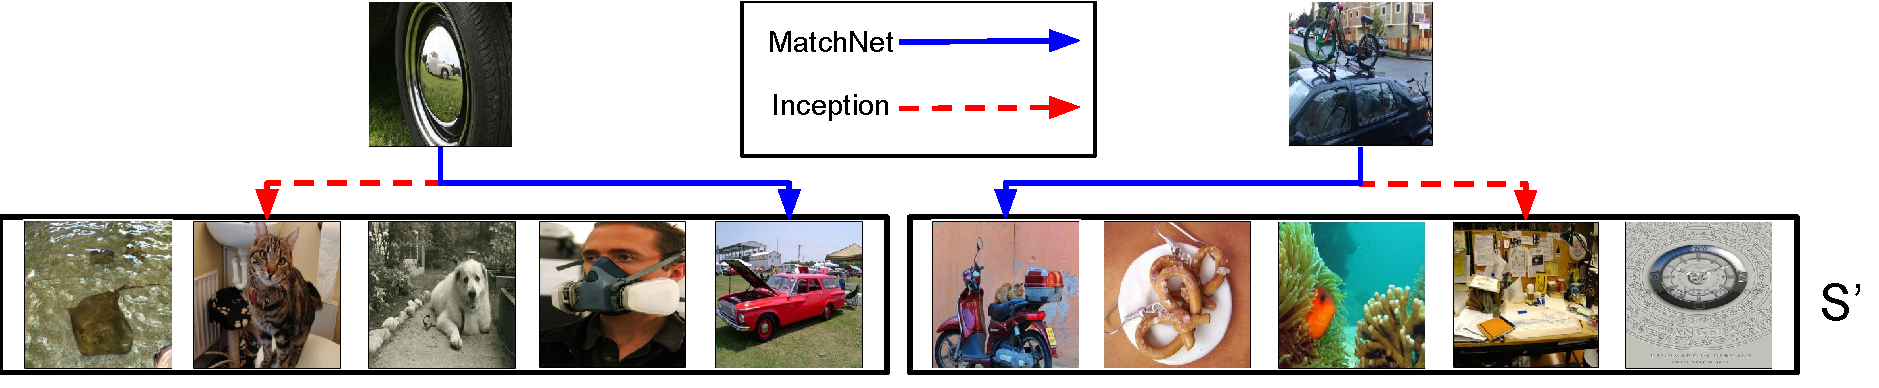
\includegraphics[width=1.0\textwidth]{figure_images}
\caption{\label{fig:imgs}Example of two 5-way problem instance on ImageNet. The images in the set $S'$ contain classes never seen during training. Our model makes far less mistakes than the Inception baseline. }
\end{figure}

\begin{table}[t]\small
\caption{
\label{tab:miniim}
Results on \emph{mini}ImageNet.
}
\begin{center}
\begin{tabular}{l@{\hskip \colspaceL}l@{\hskip \colspaceL}l@{\hskip \colspaceL}r@{\hskip \colspaceS}r@{\hskip \colspaceL}}
\toprule
\multirow{2}{*}{\b{Model}} & \multirow{2}{*}{\b{Matching Fn}} & \multirow{2}{*}{\b{Fine Tune}} & \multicolumn{2}{c}{\b{5-way Acc}} \\
~ &  ~ & ~ &1-shot & 5-shot \\
\midrule
\b{\abbr{Pixels}} & Cosine & N & \t{23.0\%} & \t{26.6\%} \\
\b{\abbr{Baseline Classifier}} & Cosine & N & \t{36.6\%} & \t{46.0\%} \\
\b{\abbr{Baseline Classifier}} & Cosine & Y & \t{36.2\%} & \t{52.2\%} \\
\b{\abbr{Baseline Classifier}} & Softmax & Y & \t{38.4\%} & \t{51.2\%} \\
\midrule
\b{\abbr{Matching Nets (Ours)}} & Cosine & N & \t{41.2\%} & \t{56.2\%} \\
\b{\abbr{Matching Nets (Ours)}} & Cosine & Y & \t{42.4\%} & \t{58.0\%} \\
\b{\abbr{Matching Nets (Ours)}} & Cosine (FCE) & N & \t{44.2\%} & \t{57.0\%} \\
\b{\abbr{Matching Nets (Ours)}} & Cosine (FCE) & Y & \b{46.6\%} & \b{60.0\%} \\
\bottomrule
\end{tabular}
\end{center}
\end{table}

Next we turned to experiments based upon full size, full scale ImageNet.
Our baseline classifier for this data set was Inception \cite{szegedy2015rethinking} trained to classify on all classes except those in the test set of classes (for \emph{rand}ImageNet) or those concerning dogs (for \emph{dogs}ImageNet).
We also compared to features from an Inception Oracle classifier trained on all classes in ImageNet, as an upper bound. Our Baseline Classifier is one of the strongest published ImageNet models at 79\% top-1 accuracy on the standard ImageNet validation set.
Instead of training Matching Networks from scratch on these large tasks, we initialised their feature extractors $f$ and $g$ with the parameters from the Inception classifier (pretrained on the appropriate subset of the data) and then further trained the resulting network on random $5$-way $1$-shot tasks from the \emph{training} data set, incorporating Full Context Embeddings and our Matching Networks and training strategy.

The results of the \emph{rand}ImageNet and \emph{dogs}ImageNet experiments are shown in Table~\ref{tab:imagenet}. The Inception Oracle (trained on all classes) performs almost perfectly when restricted to 5 classes only, which is not too surprising given its impressive top-1 accuracy. When trained solely on $\neq\!\! L_{rand}$, Matching Nets improve upon Inception by almost $6\%$ when tested on $L_{rand}$, halving the errors. Figure~\ref{fig:imgs} shows two instances of 5-way one-shot learning, where Inception fails. Looking at all the errors, Inception appears to sometimes prefer an image above all others (these images tend to be cluttered like the example in the second column, or more constant in color). Matching Nets, on the other hand, manage to recover from these outliers that sometimes appear in the support set $S'$.

Matching Nets manage to improve upon Inception on the complementary subset $\neq\!\! L_{dogs}$ (although this setup is not one-shot, as the feature extraction has been trained on these labels). However, on the much more challenging $L_{dogs}$ subset, our model degrades by $1\%$. We hypothesize this to the fact that the sampled set during training, $S$, comes from a random distribution of labels (from $\neq\!\! L_{dogs}$), whereas the testing support set $S'$ from $L_{dogs}$ contains similar classes, more akin to fine grained classification. Thus, we believe that if we adapted our training strategy to samples $S$ from fine grained sets of labels instead of sampling uniformly from the leafs of the ImageNet class tree, improvements could be attained. We leave this as future work.

\begin{table}\small
\caption{
\label{tab:imagenet}
Results on full ImageNet on \emph{rand} and \emph{dogs} one-shot tasks. Note that $\neq\!\! L_{rand}$ and $\neq\!\! L_{dogs}$ are sets of classes which are seen during training, but are provided for completeness.}
\begin{center}
\begin{tabular}{l@{\hskip \colspaceL}l@{\hskip \colspaceL}l@{\hskip \colspaceL}r@{\hskip 2.5mm}r@{\hskip 4.75mm}r@{\hskip 2.5mm}r@{}}
\toprule
\multirow{2}{*}{\b{Model}} & \multirow{2}{*}{\b{Matching Fn}} & \multirow{2}{*}{\b{Fine Tune}} & \multicolumn{4}{c}{\b{ImageNet 5-way 1-shot Acc}}\\
~ &  ~ & ~ & $L_{rand}$ & $\neq\!\! L_{rand}$ & $L_{dogs}$ & $\neq\!\! L_{dogs}$ \\
\midrule
\b{\abbr{Pixels}} & Cosine & N & \t{42.0\%} & \t{42.8\%} & \t{41.4\%} & \t{43.0\%}\\
\b{\abbr{Inception Classifier}} & Cosine & N & \t{87.6\%} & \t{92.6\%} & \b{59.8\%} & \t{90.0\%} \\
\midrule
\b{\abbr{Matching Nets (Ours)}} & Cosine (FCE) & N & \b{93.2\%} & \b{97.0\%} & \t{58.8\%} & \b{96.4\%}\\
\midrule
\b{\abbr{Inception Oracle}} & Softmax (Full) & Y (Full) & \t{$\approx 99\%$} & \t{$\approx 99\%$} & \t{$\approx 99\%$} & \t{$\approx 99\%$}\\
\bottomrule
\end{tabular}
\end{center}

\end{table}

\subsubsection{One-Shot Language Modeling}
\label{sec:ptb}
\vspace{-0.08in}

We also introduce a new one-shot language task which is analogous to those examined for images.  The task is as follows: given a query sentence with a missing word in it, and a support {\em set} of sentences which each have a missing word and a corresponding 1-hot label, choose the label from the support set that best matches the query sentence.  Here we show a single example, though note that the words on the right are not provided and the labels for the set are given as 1-hot-of-5 vectors.

\begin{tiny}
\begin{tt}
%THE SET:
\begin{tabular}{|p{0.8\textwidth}|p{0.2\textwidth}}
1. an experimental vaccine can alter the immune response of people infected with the aids virus a <blank\_token> u.s. scientist said.   
&  prominent \\
2. the show one of five new nbc <blank\_token> is the second casualty of the three networks so far this fall.     
& series \\
3. however since eastern first filed for chapter N protection march N it has consistently promised to pay creditors N cents on the <blank\_token>.
& dollar \\
4. we had a lot of people who threw in the <blank\_token> today said <unk> ellis a partner in benjamin jacobson \& sons a specialist in trading ual stock on the big board. 
& towel \\
5. it's not easy to roll out something that <blank\_token> and make it pay mr.~jacob says.
& comprehensive \\
\hline
Query: in late new york trading yesterday the <blank\_token> was quoted at N marks down from N marks late friday and at N yen down from N yen late friday. 
& dollar \\
\end{tabular}
\end{tt}
\end{tiny}

Sentences were taken from the Penn Treebank dataset \cite{marcus1993building}.  On each trial, we make sure that the set and batch are populated with sentences that are non-overlapping.  This means that we do not use words with very low frequency counts; e.g. if there is only a single sentence for a given word we do not use this data since the sentence would need to be in both the set and the batch.  As with the image tasks, each trial consisted of a 5 way choice between the classes available in the set.  We used a batch size of 20 throughout the sentence matching task and varied the set size across k=1,2,3.  We ensured that the same number of sentences were available for each class in the set. We split the words into a randomly sampled 9000 for training and 1000 for testing, and we used the standard test set to report results. Thus, neither the words nor the sentences used during test time had been seen during training.

We compared our one-shot matching model to an oracle LSTM language model (LSTM-LM) \cite{zaremba2014recurrent} trained on all the words. In this setup, the LSTM has an unfair advantage as it is not doing one-shot learning but seeing all the data -- thus, this should be taken as an upper bound.  To do so, we examined a similar setup wherein a sentence was presented to the model with a single word filled in with 5 different possible words (including the correct answer).  For each of these 5 sentences the model gave a log-likelihood and the max of these was taken to be the choice of the model.

As with the other 5 way choice tasks, chance performance on this task was 20\%.  The LSTM language model oracle achieved an upper bound of 72.8\% accuracy on the test set.  Matching Networks with a simple encoding model achieve 32.4\%, 36.1\%, 38.2\% accuracy on the task with $k=1,2,3$ examples in the set, respectively.  Future work should explore combining parametric models such as an LSTM-LM with non-parametric components such as the Matching Networks explored here.

Two related tasks are the CNN QA test of entity prediction from news articles \cite{hermann2015teaching}, and the Children's Book Test (CBT) \cite{hill2015goldilocks}.  In the CBT for example, a sequence of sentences from a book are provided as context.  In the final sentence one of the words, which has appeared in a previous sentence, is missing. The task is to choose the correct word to fill in this blank from a small set of words given as possible answers, all of which occur in the preceding sentences.  In our sentence matching task the sentences provided in the set are randomly drawn from the PTB corpus and are related to the sentences in the query batch only by the fact that they share a word. In contrast to CBT and CNN dataset, they provide only a generic rather than specific sequential context.

\section{Conclusion}
In this work, we presented the Transformer, the first sequence transduction model based entirely on attention, replacing the recurrent layers most commonly used in encoder-decoder architectures with multi-headed self-attention.

For translation tasks, the Transformer can be trained significantly faster than architectures based on recurrent or convolutional layers. On both WMT 2014 English-to-German and WMT 2014 English-to-French translation tasks, we achieve a new state of the art. In the former task our best model outperforms even all previously reported ensembles. %We also provide an indication of the broader applicability of our models through experiments on English constituency parsing.

We are excited about the future of attention-based models and plan to apply them to other tasks. We plan to extend the Transformer to problems involving input and output modalities other than text and to investigate local, restricted attention mechanisms to efficiently handle large inputs and outputs such as images, audio and video.
Making generation less sequential is another research goals of ours.

The code we used to train and evaluate our models is available at \url{https://github.com/tensorflow/tensor2tensor}.

\paragraph{Acknowledgements} We are grateful to Nal Kalchbrenner and Stephan Gouws for
their fruitful comments, corrections and inspiration.

\bibliographystyle{plain}
%\bibliography{deeplearn}
\begin{thebibliography}{10}

\bibitem{layernorm2016}
Jimmy~Lei Ba, Jamie~Ryan Kiros, and Geoffrey~E Hinton.
\newblock Layer normalization.
\newblock {\em arXiv preprint arXiv:1607.06450}, 2016.

\bibitem{bahdanau2014neural}
Dzmitry Bahdanau, Kyunghyun Cho, and Yoshua Bengio.
\newblock Neural machine translation by jointly learning to align and
  translate.
\newblock {\em CoRR}, abs/1409.0473, 2014.

\bibitem{DBLP:journals/corr/BritzGLL17}
Denny Britz, Anna Goldie, Minh{-}Thang Luong, and Quoc~V. Le.
\newblock Massive exploration of neural machine translation architectures.
\newblock {\em CoRR}, abs/1703.03906, 2017.

\bibitem{cheng2016long}
Jianpeng Cheng, Li~Dong, and Mirella Lapata.
\newblock Long short-term memory-networks for machine reading.
\newblock {\em arXiv preprint arXiv:1601.06733}, 2016.

\bibitem{cho2014learning}
Kyunghyun Cho, Bart van Merrienboer, Caglar Gulcehre, Fethi Bougares, Holger
  Schwenk, and Yoshua Bengio.
\newblock Learning phrase representations using rnn encoder-decoder for
  statistical machine translation.
\newblock {\em CoRR}, abs/1406.1078, 2014.

\bibitem{xception2016}
Francois Chollet.
\newblock Xception: Deep learning with depthwise separable convolutions.
\newblock {\em arXiv preprint arXiv:1610.02357}, 2016.

\bibitem{gruEval14}
Junyoung Chung, {\c{C}}aglar G{\"{u}}l{\c{c}}ehre, Kyunghyun Cho, and Yoshua
  Bengio.
\newblock Empirical evaluation of gated recurrent neural networks on sequence
  modeling.
\newblock {\em CoRR}, abs/1412.3555, 2014.

\bibitem{dyer-rnng:16}
Chris Dyer, Adhiguna Kuncoro, Miguel Ballesteros, and Noah~A. Smith.
\newblock Recurrent neural network grammars.
\newblock In {\em Proc. of NAACL}, 2016.

\bibitem{JonasFaceNet2017}
Jonas Gehring, Michael Auli, David Grangier, Denis Yarats, and Yann~N. Dauphin.
\newblock Convolutional sequence to sequence learning.
\newblock {\em arXiv preprint arXiv:1705.03122v2}, 2017.

\bibitem{graves2013generating}
Alex Graves.
\newblock Generating sequences with recurrent neural networks.
\newblock {\em arXiv preprint arXiv:1308.0850}, 2013.

\bibitem{he2016deep}
Kaiming He, Xiangyu Zhang, Shaoqing Ren, and Jian Sun.
\newblock Deep residual learning for image recognition.
\newblock In {\em Proceedings of the IEEE Conference on Computer Vision and
  Pattern Recognition}, pages 770--778, 2016.

\bibitem{hochreiter2001gradient}
Sepp Hochreiter, Yoshua Bengio, Paolo Frasconi, and J{\"u}rgen Schmidhuber.
\newblock Gradient flow in recurrent nets: the difficulty of learning long-term
  dependencies, 2001.

\bibitem{hochreiter1997}
Sepp Hochreiter and J{\"u}rgen Schmidhuber.
\newblock Long short-term memory.
\newblock {\em Neural computation}, 9(8):1735--1780, 1997.

\bibitem{huang-harper:2009:EMNLP}
Zhongqiang Huang and Mary Harper.
\newblock Self-training {PCFG} grammars with latent annotations across
  languages.
\newblock In {\em Proceedings of the 2009 Conference on Empirical Methods in
  Natural Language Processing}, pages 832--841. ACL, August 2009.

\bibitem{jozefowicz2016exploring}
Rafal Jozefowicz, Oriol Vinyals, Mike Schuster, Noam Shazeer, and Yonghui Wu.
\newblock Exploring the limits of language modeling.
\newblock {\em arXiv preprint arXiv:1602.02410}, 2016.

\bibitem{extendedngpu}
{\L}ukasz Kaiser and Samy Bengio.
\newblock Can active memory replace attention?
\newblock In {\em Advances in Neural Information Processing Systems, ({NIPS})},
  2016.

\bibitem{neural_gpu}
\L{}ukasz Kaiser and Ilya Sutskever.
\newblock Neural {GPU}s learn algorithms.
\newblock In {\em International Conference on Learning Representations
  ({ICLR})}, 2016.

\bibitem{NalBytenet2017}
Nal Kalchbrenner, Lasse Espeholt, Karen Simonyan, Aaron van~den Oord, Alex
  Graves, and Koray Kavukcuoglu.
\newblock Neural machine translation in linear time.
\newblock {\em arXiv preprint arXiv:1610.10099v2}, 2017.

\bibitem{structuredAttentionNetworks}
Yoon Kim, Carl Denton, Luong Hoang, and Alexander~M. Rush.
\newblock Structured attention networks.
\newblock In {\em International Conference on Learning Representations}, 2017.

\bibitem{kingma2014adam}
Diederik Kingma and Jimmy Ba.
\newblock Adam: A method for stochastic optimization.
\newblock In {\em ICLR}, 2015.

\bibitem{Kuchaiev2017Factorization}
Oleksii Kuchaiev and Boris Ginsburg.
\newblock Factorization tricks for {LSTM} networks.
\newblock {\em arXiv preprint arXiv:1703.10722}, 2017.

\bibitem{lin2017structured}
Zhouhan Lin, Minwei Feng, Cicero Nogueira~dos Santos, Mo~Yu, Bing Xiang, Bowen
  Zhou, and Yoshua Bengio.
\newblock A structured self-attentive sentence embedding.
\newblock {\em arXiv preprint arXiv:1703.03130}, 2017.

\bibitem{multiseq2seq}
Minh-Thang Luong, Quoc~V. Le, Ilya Sutskever, Oriol Vinyals, and Lukasz Kaiser.
\newblock Multi-task sequence to sequence learning.
\newblock {\em arXiv preprint arXiv:1511.06114}, 2015.

\bibitem{luong2015effective}
Minh-Thang Luong, Hieu Pham, and Christopher~D Manning.
\newblock Effective approaches to attention-based neural machine translation.
\newblock {\em arXiv preprint arXiv:1508.04025}, 2015.

\bibitem{marcus1993building}
Mitchell~P Marcus, Mary~Ann Marcinkiewicz, and Beatrice Santorini.
\newblock Building a large annotated corpus of english: The penn treebank.
\newblock {\em Computational linguistics}, 19(2):313--330, 1993.

\bibitem{mcclosky-etAl:2006:NAACL}
David McClosky, Eugene Charniak, and Mark Johnson.
\newblock Effective self-training for parsing.
\newblock In {\em Proceedings of the Human Language Technology Conference of
  the NAACL, Main Conference}, pages 152--159. ACL, June 2006.

\bibitem{decomposableAttnModel}
Ankur Parikh, Oscar Täckström, Dipanjan Das, and Jakob Uszkoreit.
\newblock A decomposable attention model.
\newblock In {\em Empirical Methods in Natural Language Processing}, 2016.

\bibitem{paulus2017deep}
Romain Paulus, Caiming Xiong, and Richard Socher.
\newblock A deep reinforced model for abstractive summarization.
\newblock {\em arXiv preprint arXiv:1705.04304}, 2017.

\bibitem{petrov-EtAl:2006:ACL}
Slav Petrov, Leon Barrett, Romain Thibaux, and Dan Klein.
\newblock Learning accurate, compact, and interpretable tree annotation.
\newblock In {\em Proceedings of the 21st International Conference on
  Computational Linguistics and 44th Annual Meeting of the ACL}, pages
  433--440. ACL, July 2006.

\bibitem{press2016using}
Ofir Press and Lior Wolf.
\newblock Using the output embedding to improve language models.
\newblock {\em arXiv preprint arXiv:1608.05859}, 2016.

\bibitem{sennrich2015neural}
Rico Sennrich, Barry Haddow, and Alexandra Birch.
\newblock Neural machine translation of rare words with subword units.
\newblock {\em arXiv preprint arXiv:1508.07909}, 2015.

\bibitem{shazeer2017outrageously}
Noam Shazeer, Azalia Mirhoseini, Krzysztof Maziarz, Andy Davis, Quoc Le,
  Geoffrey Hinton, and Jeff Dean.
\newblock Outrageously large neural networks: The sparsely-gated
  mixture-of-experts layer.
\newblock {\em arXiv preprint arXiv:1701.06538}, 2017.

\bibitem{srivastava2014dropout}
Nitish Srivastava, Geoffrey~E Hinton, Alex Krizhevsky, Ilya Sutskever, and
  Ruslan Salakhutdinov.
\newblock Dropout: a simple way to prevent neural networks from overfitting.
\newblock {\em Journal of Machine Learning Research}, 15(1):1929--1958, 2014.

\bibitem{sukhbaatar2015}
Sainbayar Sukhbaatar, Arthur Szlam, Jason Weston, and Rob Fergus.
\newblock End-to-end memory networks.
\newblock In C.~Cortes, N.~D. Lawrence, D.~D. Lee, M.~Sugiyama, and R.~Garnett,
  editors, {\em Advances in Neural Information Processing Systems 28}, pages
  2440--2448. Curran Associates, Inc., 2015.

\bibitem{sutskever14}
Ilya Sutskever, Oriol Vinyals, and Quoc~VV Le.
\newblock Sequence to sequence learning with neural networks.
\newblock In {\em Advances in Neural Information Processing Systems}, pages
  3104--3112, 2014.

\bibitem{DBLP:journals/corr/SzegedyVISW15}
Christian Szegedy, Vincent Vanhoucke, Sergey Ioffe, Jonathon Shlens, and
  Zbigniew Wojna.
\newblock Rethinking the inception architecture for computer vision.
\newblock {\em CoRR}, abs/1512.00567, 2015.

\bibitem{KVparse15}
{Vinyals {\&} Kaiser}, Koo, Petrov, Sutskever, and Hinton.
\newblock Grammar as a foreign language.
\newblock In {\em Advances in Neural Information Processing Systems}, 2015.

\bibitem{wu2016google}
Yonghui Wu, Mike Schuster, Zhifeng Chen, Quoc~V Le, Mohammad Norouzi, Wolfgang
  Macherey, Maxim Krikun, Yuan Cao, Qin Gao, Klaus Macherey, et~al.
\newblock Google's neural machine translation system: Bridging the gap between
  human and machine translation.
\newblock {\em arXiv preprint arXiv:1609.08144}, 2016.

\bibitem{DBLP:journals/corr/ZhouCWLX16}
Jie Zhou, Ying Cao, Xuguang Wang, Peng Li, and Wei Xu.
\newblock Deep recurrent models with fast-forward connections for neural
  machine translation.
\newblock {\em CoRR}, abs/1606.04199, 2016.

\bibitem{zhu-EtAl:2013:ACL}
Muhua Zhu, Yue Zhang, Wenliang Chen, Min Zhang, and Jingbo Zhu.
\newblock Fast and accurate shift-reduce constituent parsing.
\newblock In {\em Proceedings of the 51st Annual Meeting of the ACL (Volume 1:
  Long Papers)}, pages 434--443. ACL, August 2013.

\end{thebibliography}
%\newpage
\pagebreak
\section*{Attention Visualizations}\label{sec:viz-att}
\begin{figure*}[h]
{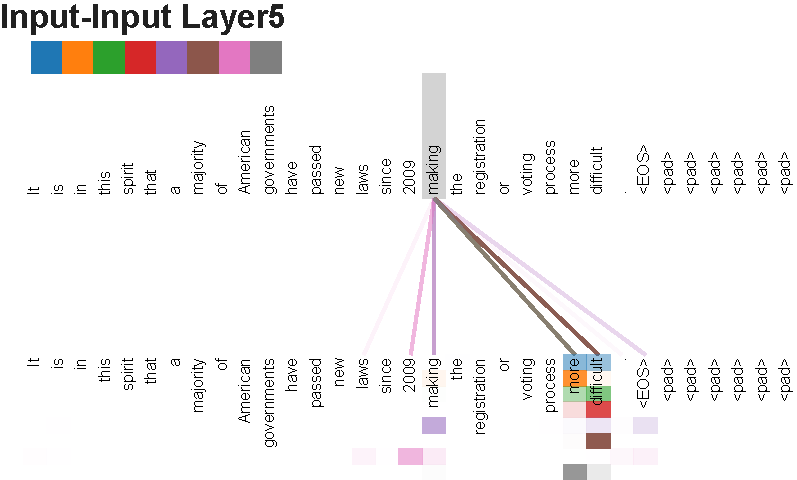
\includegraphics[width=\textwidth, trim=0 0 0 36, clip]{./vis/making_more_difficult5_new.pdf}}
\caption{An example of the attention mechanism following long-distance dependencies in the encoder self-attention in layer 5 of 6. Many of the attention heads attend to a distant dependency of the verb `making', completing the phrase `making...more difficult'.  Attentions here shown only for the word `making'. Different colors represent different heads. Best viewed in color.}
\end{figure*}

\begin{figure*}
{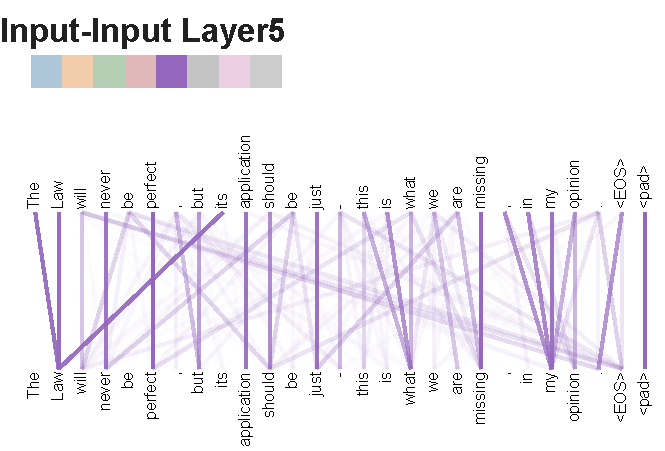
\includegraphics[width=\textwidth, trim=0 0 0 45, clip]{./vis/anaphora_resolution_new.pdf}}
{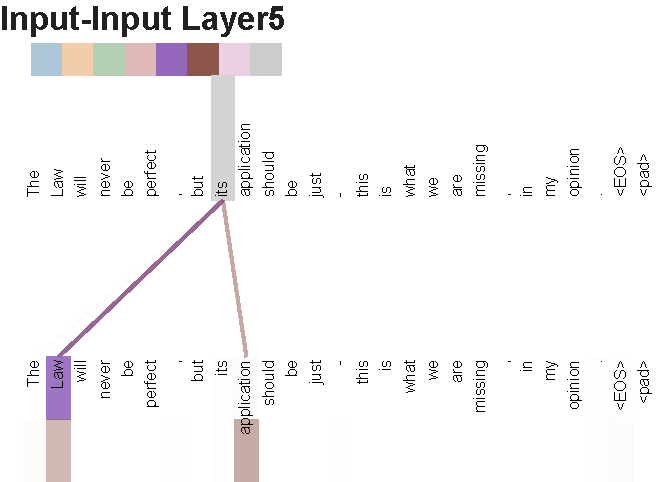
\includegraphics[width=\textwidth, trim=0 0 0 37, clip]{./vis/anaphora_resolution2_new.pdf}}
\caption{Two attention heads, also in layer 5 of 6, apparently involved in anaphora resolution. Top: Full attentions for head 5. Bottom: Isolated attentions from just the word `its' for attention heads 5 and 6. Note that the attentions are very sharp for this word.}
\end{figure*}

\begin{figure*}
{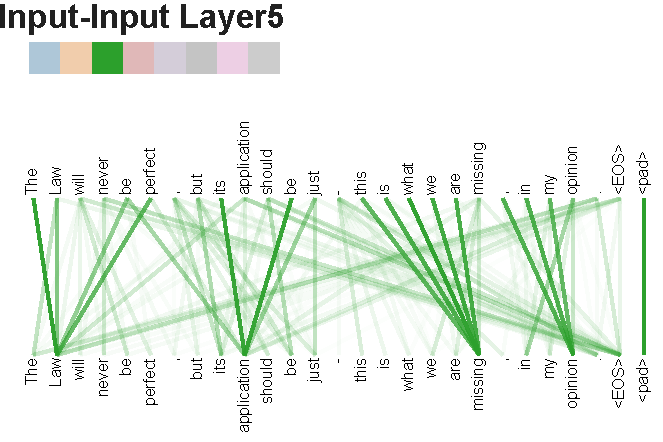
\includegraphics[width=\textwidth, trim=0 0 0 36, clip]{./vis/attending_to_head_new.pdf}}
{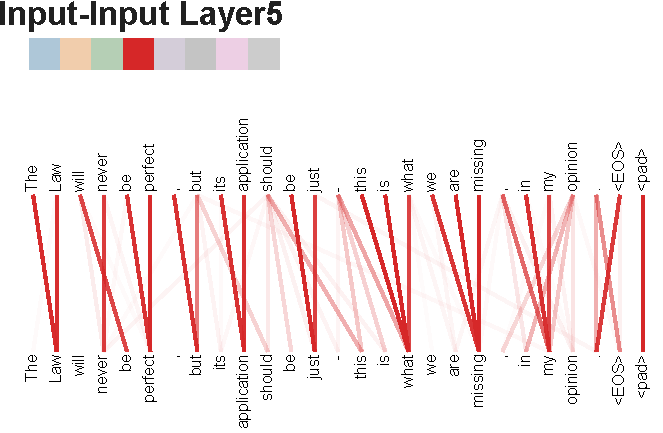
\includegraphics[width=\textwidth, trim=0 0 0 36, clip]{./vis/attending_to_head2_new.pdf}}
\caption{Many of the attention heads exhibit behaviour that seems related to the structure of the sentence. We give two such examples above, from two different heads from the encoder self-attention at layer 5 of 6. The heads clearly learned to perform different tasks.}
\end{figure*}

%\appendix
%\newpage
%\pagebreak
\section*{Two Feed-Forward Layers = Attention over Parameters}\label{sec:parameter_attention}

In addition to attention layers, our model contains position-wise feed-forward networks (Section \ref{sec:ffn}), which consist of two linear transformations with a ReLU activation in between.  In fact, these networks too can be seen as a form of attention.  Compare the formula for such a network with the formula for a simple dot-product attention layer (biases and scaling factors omitted):

\begin{align*}
    FFN(x, W_1, W_2) = ReLU(xW_1)W_2 \\
    A(q, K, V) = Softmax(qK^T)V
\end{align*}

Based on the similarity of these formulae, the two-layer feed-forward network can be seen as a kind of attention, where the keys and values are the rows of the trainable parameter matrices $W_1$ and $W_2$, and where we use ReLU instead of Softmax in the compatibility function.

%the compatablity function is $compat(q, k_i) = ReLU(q \cdot k_i)$ instead of $Softmax(qK_T)_i$.

Given this similarity, we experimented with replacing the position-wise feed-forward networks with attention layers similar to the ones we use everywhere else our model. The multi-head-attention-over-parameters sublayer is identical to the multi-head attention described in \ref{sec:multihead}, except that the "keys" and "values" inputs to each attention head are trainable model parameters, as opposed to being linear projections of a previous layer.  These parameters are scaled up by a factor of $\sqrt{d_{model}}$ in order to be more similar to activations.

In our first experiment, we replaced each position-wise feed-forward network with a multi-head-attention-over-parameters sublayer with $h_p=8$ heads, key-dimensionality $d_{pk}=64$, and value-dimensionality $d_{pv}=64$, using $n_p=1536$ key-value pairs for each attention head.  The sublayer has a total of $2097152$ parameters, including the parameters in the query projection and the output projection.  This matches the number of parameters in the position-wise feed-forward network that we replaced.  While the theoretical amount of computation is also the same, in practice, the attention version caused the step times to be about 30\% longer.

In our second experiment, we used $h_p=8$ heads, and $n_p=512$ key-value pairs for each attention head, again matching the total number of parameters in the base model.

Results for the first experiment were slightly worse than for the base model, and results for the second experiment were slightly better, see Table~\ref{tab:parameter_attention}.

\begin{table}[h]
\caption{Replacing the position-wise feed-forward networks with multihead-attention-over-parameters produces similar results to the base model.  All metrics are on the English-to-German translation development set, newstest2013.}
\label{tab:parameter_attention}
\begin{center}
\vspace{-2mm}
%\scalebox{1.0}{
\begin{tabular}{c|cccccc|cccc}
\hline\rule{0pt}{2.0ex}
 & \multirow{2}{*}{$\dmodel$} & \multirow{2}{*}{$\dff$} &
\multirow{2}{*}{$h_p$} & \multirow{2}{*}{$d_{pk}$} & \multirow{2}{*}{$d_{pv}$} &
 \multirow{2}{*}{$n_p$} &
 PPL & BLEU & params & training\\
 & & & & & &  & (dev) & (dev) & $\times10^6$ & time \\
\hline\rule{0pt}{2.0ex}
base & 512 & 2048 & & & & & 4.92 & 25.8 & 65 & 12 hours\\
\hline\rule{0pt}{2.0ex}
AOP$_1$ & 512 & & 8 & 64 & 64 & 1536 & 4.92& 25.5  & 65 & 16 hours\\
AOP$_2$ & 512 & & 16 & 64 & 64 & 512 & \textbf{4.86} & \textbf{25.9}  & 65 & 16 hours \\
\hline
\end{tabular}
%}
\end{center}
\end{table}


%\section*{Justfication of the Scaling Factor in Dot-product Attention}

In Section~\ref{sec:scaled-dot-prod}, we introduced Scaled dot-product attention, where we scale down the dot products by $\sqrt{d_k}$.   In this section, we will give a rough justification of this scaling factor.  If we assume that $q$ and $k$ are $d_k$-dimensional vectors whose components are independent random variables with mean $0$ and variance $1$, then their dot product, $q \cdot k = \sum_{i=1}^{d_k} u_iv_i$, has mean $0$ and variance $d_k$.  Since we would prefer these values to have variance $1$, we divide by $\sqrt{d_k}$.  



%For any two $d_k$-dimension vectors $\vec{u}$ and $\vec{v}$, whose dimensions are independent, the mean and variance of the dot product will be the summation of the product of means and variances over the dimensions, that is, $E[<\vec{u},\vec{v}>] = \sum_{i=1}^{d_k} E[u_i]E[v_i]$, and $E[(<\vec{u},\vec{v}>-E[<\vec{u},\vec{v}>])^2] = \sum_{i=1}^{d_k} E[({u_i}-E[u_i])^2] E[({v_i}-E[v_i])^2]$. Layer norm encourages the mean and variance of each dimension to be $0$ and $1$ respectively, resultig in the dot product having mean $0$ and $d_k$ respectively. Therefore, scaling by $\sqrt{d_k}$ encourages the logits to be normalized as well. 

\iffalse

In this section, we will give a rough justification of this scaling factor, that is, we will show that for any two vectors, $\vec{u}$ and $\vec{v}$, whose variance and mean are $1$ and $0$ respectively, the variance and the mean of the dot product are $d_k$ and $0$ respectively. Therefore, dividing by $\sqrt{d_k}$ ensures that each component of the attention logits are normalized. The repeated layer norms at each transformer layer encourage $\vec{u}$ and $\vec{v}$ to be normalized. 


\begin{align*}
    E[<\vec{u},\vec{v}>] & =  \sum_k E[u_i v_i] &\text{By linearity of expectation} \\
    & =\sum_k E[u_i]E[v_i] & \text{Assuming independence} \\
    & = 0
\end{align*}

\begin{align*}
    E[(<\vec{u},\vec{v}>-E[<\vec{u},\vec{v}>])^2]  & = E[(<\vec{u},\vec{v}>)^2] - E[<\vec{u},\vec{v}>]^2 \\
    & = E[(<\vec{u},\vec{v}>)^2] \\
    & =  \sum_k E[{u_i}^2] E[{v_i}^2] &\text{By linearity of expectation and indepedence} \\
    & = d_k
\end{align*}


\fi

\end{document}
